\pagestyle{milan}
\section{Sensitivitätsanalyse der Modellparameter}\label{sec:sesitivitaetsanalyse}
In diesem Abschnitt wird eine Parameter- und Sensitivitätsanalyse durchgeführt. 
Es wird dabei die Auswirkung von der Varianz von bestimmten Modellparametern auf die Varianz der Ausgangsparameter untersucht.

Ziel der Sensitivitätsanalyse ist es, wichtige Parameter zu identifizieren und daraus eine Optimierung der Parameter zu ermitteln.

Das Ergebnis der Sensitivitätsanalyse dient zum weiteren Verständnis des mathematischen Modells bzw. dem zugrundeliegenden Simulationsmodell.
\subsection{Lokale und globale Sensitivitätsanalyse}

Die verschiedenen Verfahren zur Sensitivitätsanalyse lassen sich in drei Kategorien einteilen: Lokale, globale Sensitivitätsanalyse und der sogenannten Screening-Methode.

Bei der lokalen Sensitivitätsanalyse wird für bestimmte Werte der Ausgangsgrößen der Einfluss der Eingangsgrößen untersucht. Dabei wird immer ein Parameter variiert und die restlichen konstant gehalten (One-At-a-Time-Methode, OAT).
Die Sensitivitätsanalyse wird so für jeden Parameter einzeln durchgeführt und abschließend kann die spezifische Sensitivität der einzelnen Parameter ermittelt werden.
Mathematisch entspricht dies den partiellen Ableitungen der Parameter bezüglich der Ausgangsgrößen

\subsubsection*{One-factor-at-a-time ($\pm \SI{20}{\percent}, \pm 1\, \sigma$)}

\begin{equation}
    sensitivity=\frac{\Delta Y}{\Delta X_{i}} \quad \textrm{Für jeden Parameter}\,X_i, i=1,\dots,n
\end{equation}
\begin{itemize}
    \item Nur lokale Variation um Arbeitspunkt 
    \item keine Korrelation zwischen Parametern
    \item Standardabweichung benötigt Annahme zur Distribution und überspannt nicht den gesamten Wertebereich
\end{itemize}

\subsubsection*{Ausdruck als Partial-Ableitung}
\begin{equation}
    sensitivity=\frac{\partial Y}{\partial X_i}
\end{equation}
Für die Analytische Lösung wird ein lineares Modell benötigt. Die Linearisierung wurde zwar in Kap. \ref{sec:LMI} für dieses Modell durchgeführt, jeddoch soll im Rahmen dieser Arbeit nicht weiter darauf eingeganen werden.
\subsubsection*{Globale Sensitivitätsanalyse}
Bei der globlan Sensitivitätsanalyse wird, im gegensatz zur lokalen Sensitivitätsanalyse nicht nur ein Parameter variiert, sondern alle Parameter gleichzeitig.
Dies macht es möglich auch Abhängigkeiten unter den Parametern zu berücksichtigen. \\
Ebenso werden die Parameter nich nur über einen kelien lokalen Bereich verrändert, sodner über den gesammten Definitionsbereich.
Dieser ist bei Physikalischen Modellen meist nicht bekannt, sodass hierfür eine statistische Verteilung der Parameter angenommen werden muss.
Dennoch sollte die Verteilung so gewählt werden, dass sie den tatsächlichen physikalische möglichen Verteilungen möglichst nahe kommt.

Allerdings ist die globale Sensitivitätsanalyse sehr aufwendig und kann nur für kleine Modelle durchgeführt werden.\\

\textbf{Monte Carlo Methode:}
Die Monte Carlo Methode ist eine statistische Methode, die zur Lösung von Problemen mit mehreren Variablen eingesetzt wird.
Sie generiert einen zufälligen Parameterraum und berechnet für diesen die Ausgangsgrößen.
Die so enstehehnden Scatterplots können dann zur eifnachen graphischen Analyse der Parameter verwendet werden.


\subsection{Parameter}
Aus den gesamten Modellparametern des Schwungradpendels (\ref{tab:Tabelle1.1}) werden folgende Parameter untersucht:
\begin{itemize}
    \item $C1,\, C2$
    \item $J1,\, J2$
    \item $m1,\, m2$
    \item $l1,\, l2$
    \item $V_m$
\end{itemize}
Es wird dabei die Auswirkung der Varianz genannter Parameter auf folgende Modellgrößen untersucht:
\begin{itemize}
    \item Schwungrad Geschwindigkeit: $\dot\varphi$
    \item Schwungrad Beschleunigung: $\ddot\varphi$
    \item Pendel Winkel: $\Theta$
    \item Pendel Geschwindigkeit: $\dot\Theta$
    \item Pendel Beschleunigung: $\ddot\Theta$
    \item Motor Moment: $\tau$
\end{itemize}


\subsection*{Modellantwort auf Eingangssprung}

Um ein besseres Verständnis des Modells zu erlangen, wird die Antwort wichtiger Parameter auf einen Sprung der Motorspannung $V_{\mathrm{m}}$ betrachtet.
Zugrundeliegenden ist das in\,\ref{cap:nichtlinearesZustandsraummodell} entwickelte Simulink-Modell.

Der Eingangsprung der Motorspannung erfolgt in den Größen: $V_{\mathrm{m}}=\SI{5}{\volt},\SI{10}{\volt},\SI{15}{\volt},\SI{20}{\volt}$.
Das Pendel befindet sich dabei in Ruhelage ($\Theta=\SI{180}{\degree}$). 
Ein Eingangsprung führt zu einem Moment an der Motorwelle, welches das Schwungrad und das Pendel in Bewegung versetzt.\\

\begin{wrapfigure}{l}{.5\textwidth}
    \captionsetup[subfigure]{justification=centering,font=footnotesize}
    \begin{subfigure}[b]{0.49\linewidth}
        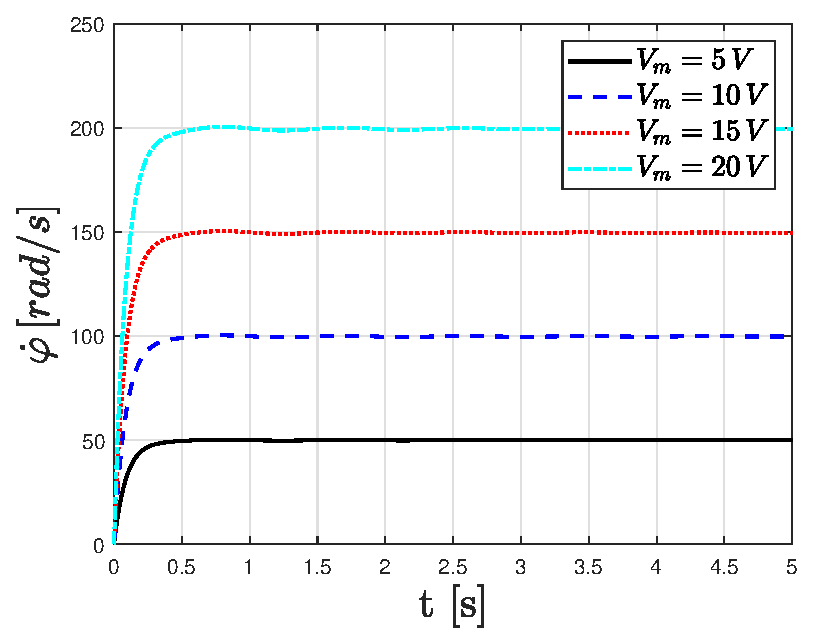
\includegraphics[width=\linewidth]{Bilder/5_sensi/fig/Vm_sprung/phi_punkt.eps}
        \caption{Schwungrad Geschwindigkeit}
        \label{fig:Vm_sprung_phi_punkt}
    \end{subfigure}
    \begin{subfigure}[b]{0.49 \linewidth}
        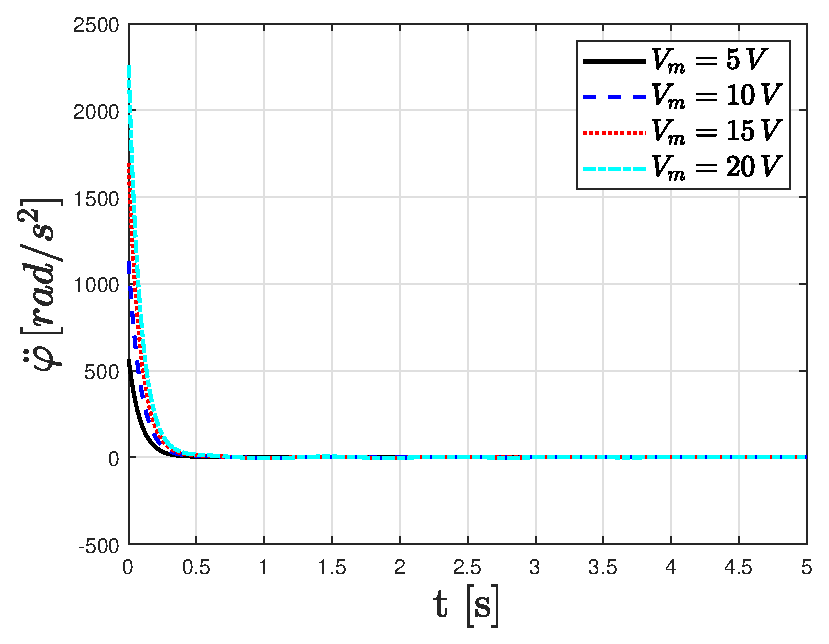
\includegraphics[width=\linewidth]{Bilder/5_sensi/fig/Vm_sprung/phi_punkt_punkt.eps}
        \caption{Schwungrad Beschleunigung}
        \label{fig:Vm_sprung_phi_punkt_punkt}
    \end{subfigure}
    \begin{subfigure}[b]{0.49 \linewidth}
        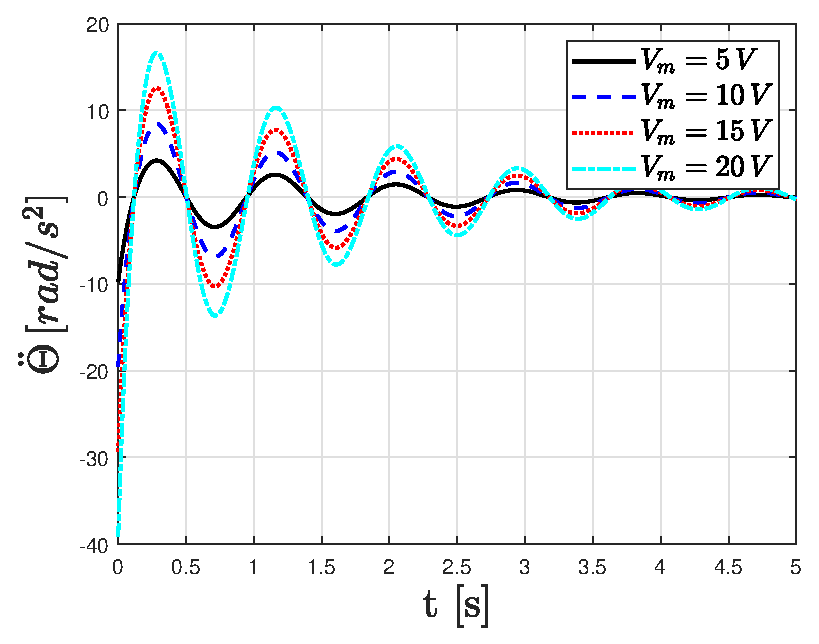
\includegraphics[width=\linewidth]{Bilder/5_sensi/fig/Vm_sprung/theta_punkt_punkt.eps}
        \caption{Pendel Beschleunigung}
        \label{fig:Vm_sprung_theta_punkt_punkt}
    \end{subfigure}
    \begin{subfigure}[b]{0.49\linewidth}
        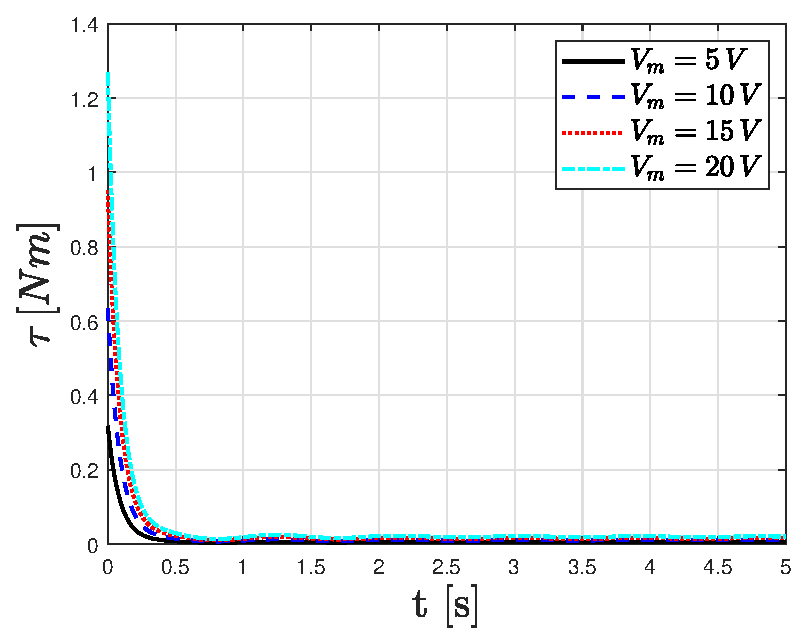
\includegraphics[width=\linewidth]{Bilder/5_sensi/fig/Vm_sprung/tau.eps}
        \caption{Motor Moment}
        \label{fig:Vm_sprung_tau}
    \end{subfigure}
    \begin{subfigure}[b]{0.49\linewidth}
        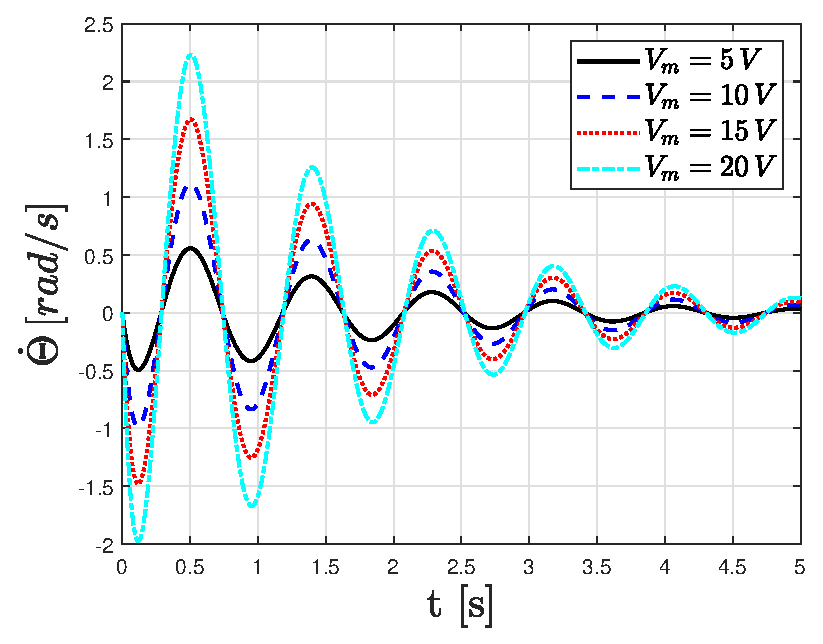
\includegraphics[width=\linewidth]{Bilder/5_sensi/fig/Vm_sprung/theta_punkt.eps}
        \caption{Pendel Geschwindigkeit}
        \label{fig:Vm_sprung_theta_punkt}      
    \end{subfigure}
    \begin{subfigure}[b]{0.49\linewidth}
        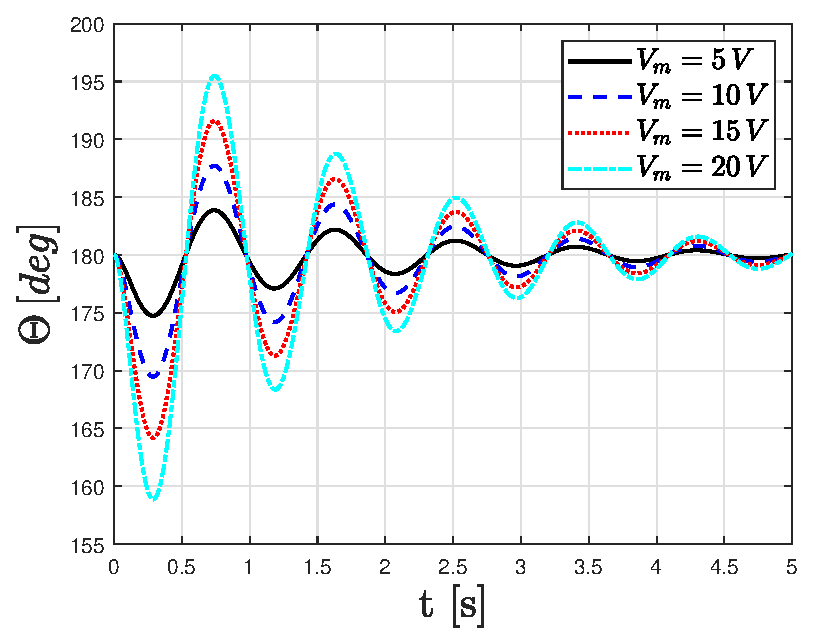
\includegraphics[width=\linewidth]{Bilder/5_sensi/fig/Vm_sprung/theta.eps}
        \caption{Pendel Winkel}
        \label{fig:Vm_sprung_theta}
    \end{subfigure}
        \caption{Modellantwort auf Eingangssprung der Motorspannung}
\end{wrapfigure}
In Abb.\,\ref{fig:Vm_sprung_phi_punkt} ist zu erkennen, dass der stabile Zustand der Endgeschwindigkeit des Schwungrades ungefähr zur selber Zeit ($t=\SI{0.5}{\s}$) erreicht wird.
Die dabei erreichte Endgeschwindigkeit ist direkt abhängig von der angelegten Motorspannung $V_m$.\\
Das Maximum des Motormomentes hängt dabei ebenso von der Höhe der angelegten Motorspannung $V_m$ ab (Abb. \ref{fig:Vm_sprung_tau}).
Das Moment erzeugt dabei eine Beschleunigung des Schwungrades (Abb. \ref{fig:Vm_sprung_phi_punkt_punkt}), die ebenso durch das Moment in Abhängigkeit zur Höhe des angelegten Motorstroms steht.

Das Pendel wird durch das Moment in Bewegung versetzt und schwingt in Eigenfrequenz (Abb. \ref{fig:Vm_sprung_theta}). 
Die Amplitude der Pendelbewegung ist dabei abhängig von der Höhe der angelegten Motorspannung $V_m$.

Die Pendelgeschwindigkeit (Abb. \ref{fig:Vm_sprung_theta_punkt}) hat ihren Nulldurchgang beim maximaler Amplitude des Pendelwinkels (Abb. \ref{fig:Vm_sprung_tau}), wobei die maximale Pendelgeschwindigkeit bei $\tau=\SI{180}{\degree}$ erreicht wird.

Nach Erreichen der Endgeschwindigkeit des Schwungrades, geht die Beschleunigung gegen null und das Motormoment gleicht dem Reibungsmoment (Abb. \ref{fig:Vm_sprung_tau}).
Das Pendel ist ab diesen Moment nur noch durch die Gravitation beeinflusst und schwing so lange bis es in Ruheposition zurückkehrt.

\subsection*{Einfluss der Länge des Pendels zum Massezentrum des Schwungrades (l2)}
Die Länge von der Aufhängung des Pendels bis zum Masseschwerpunkt des Schwungrades ($l2$) ist ein weiterer Parameter, er im Folgenden untersucht wird.
In den Simulationen (Abb. \ref{fig:l2}) wurde der Parameter $l2$ von $\SI{0.1}{\m}$ bis $\SI{1.5}{\m}$ variiert.
Die Motorspannung wird dabei auf \SI{10}{\volt} gesetzt und die anderen Parameter werden ebenfalls auf die Standardwerte in Tab. \ref{tab:Tabelle1.1} festgelegt.
\pagebreak

\begin{wrapfigure}{l}{.5\textwidth}
    \captionsetup[subfigure]{justification=centering,font=footnotesize}
    \begin{subfigure}[b]{0.49\linewidth}
        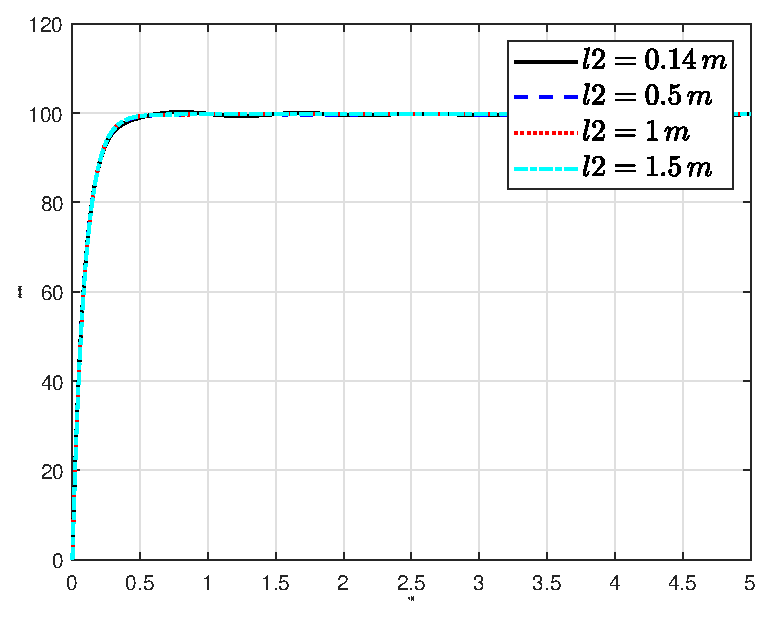
\includegraphics[width=\linewidth]{Bilder/5_sensi/fig/l2/phi_punkt.eps}
        \caption{Schwungrad Geschwindigkeit}
        \label{fig:l2_phi_punkt}
    \end{subfigure}
    \begin{subfigure}[b]{0.49 \linewidth}
        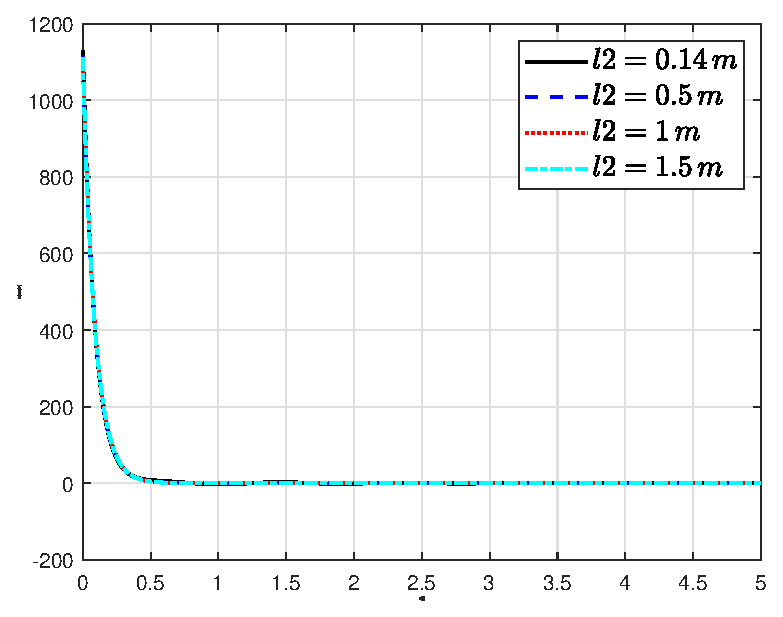
\includegraphics[width=\linewidth]{Bilder/5_sensi/fig/l2/phi_punkt_punkt.eps}
        \caption{Schwungrad Beschleunigung}
        \label{fig:l2_phi_punkt_punkt}
    \end{subfigure}
    \begin{subfigure}[b]{0.49 \linewidth}
        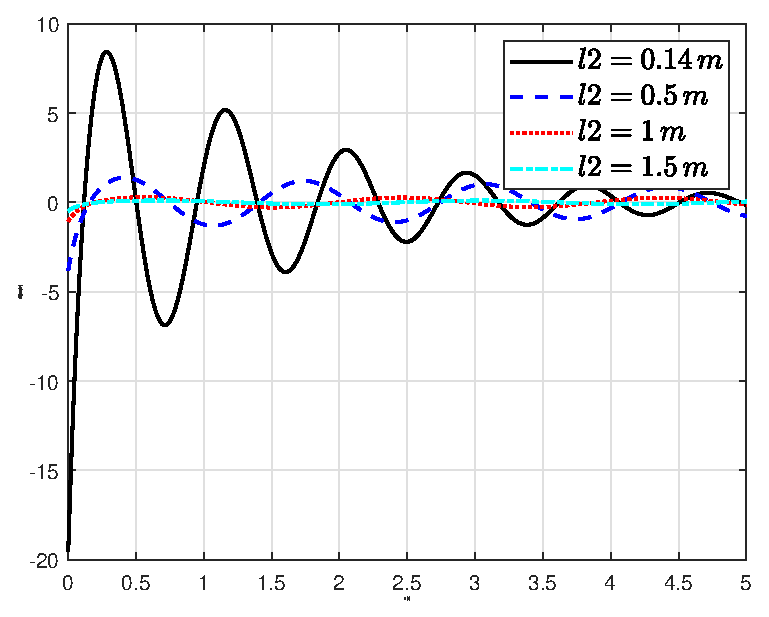
\includegraphics[width=\linewidth]{Bilder/5_sensi/fig/l2/theta_punkt_punkt.eps}
        \caption{Pendel Beschleunigung}
        \label{fig:l2_theta_punkt_punkt}
    \end{subfigure}
    \begin{subfigure}[b]{0.49\linewidth}
        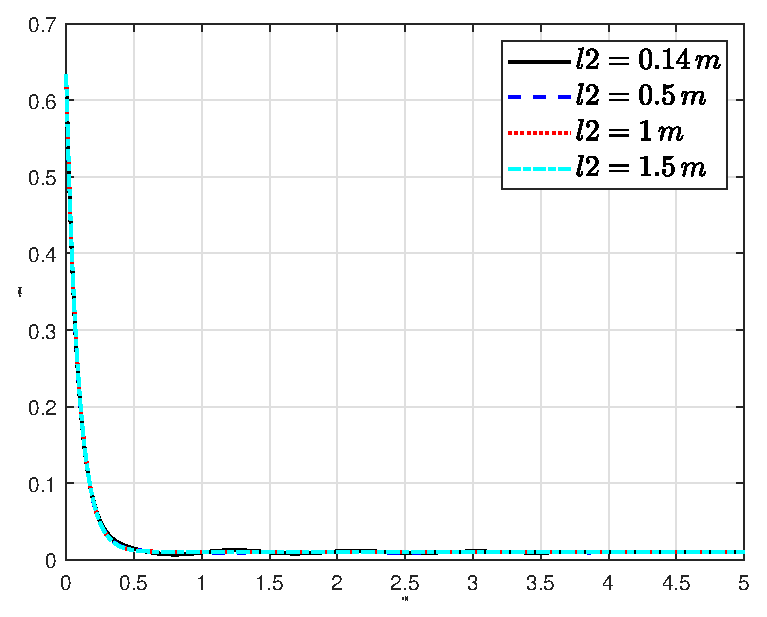
\includegraphics[width=\linewidth]{Bilder/5_sensi/fig/l2/tau.eps}
        \caption{Motor Moment}
        \label{fig:l2_tau}
    \end{subfigure}
    \begin{subfigure}[b]{0.49\linewidth}
        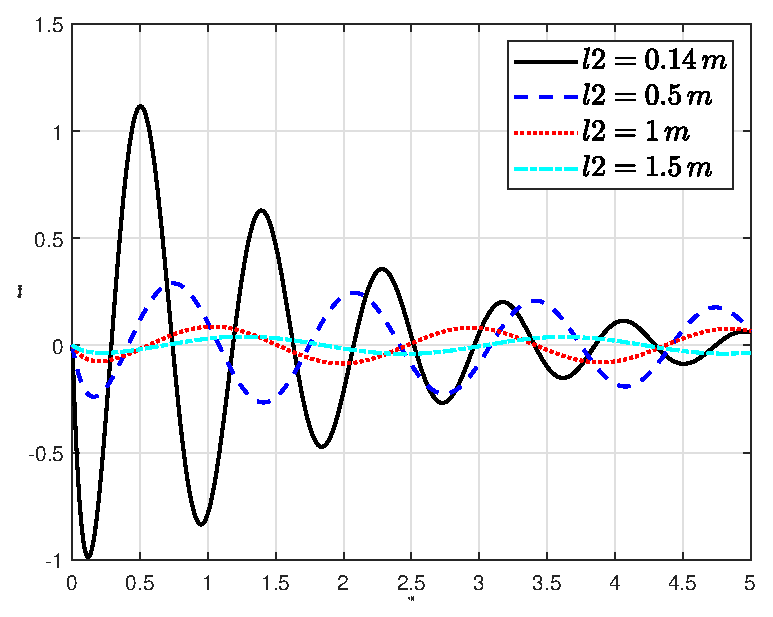
\includegraphics[width=\linewidth]{Bilder/5_sensi/fig/l2/theta_punkt.eps}
        \caption{Pendel Geschwindigkeit}
        \label{fig:l2_theta_punkt}      
    \end{subfigure}
    \begin{subfigure}[b]{0.49\linewidth}
        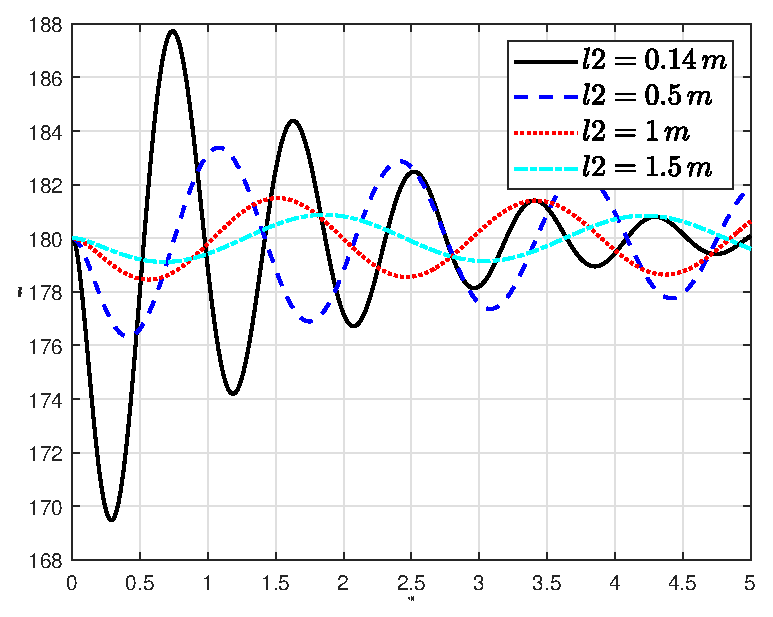
\includegraphics[width=\linewidth]{Bilder/5_sensi/fig/l2/theta.eps}
        \caption{Pendel Winkel}
        \label{fig:l2_theta}
    \end{subfigure}
        \caption{Modellantwort auf Varianz des Parameters: $l2$}
        \label{fig:l2}
\end{wrapfigure}
Abbildung \ref{fig:l2_phi_punkt}, \ref{fig:l2_phi_punkt}, \ref{fig:l2_tau} zeigen keine Abweichung, was zeigt das der Parameter $l2$ keinen Einfluss auf die Modellgrößen $\dot\varphi,\ddot\varphi,\tau$ hat.
Es ist jedoch ein Einfluss auf die Parameter $\Theta,\dot\Theta,\ddot\Theta$ (Abb. \ref{fig:l2_theta}\ref{fig:l2_theta_punkt}\ref{fig:l2_theta_punkt_punkt}) zu erkennen. 

Bei kleinerer Länge $l2$ erhöht sich die Amplitude des Winkels $\Theta$ sowie dessen Geschwindigkeit $\dot\Theta$ und Beschleunigung $\ddot\Theta$. 

Ebenso ist zu erkennen, dass sich die Eigenfrequenz, mit der das Pendel schwing, verändert.
Je größer die Länge $l2$ ist, desto größeres Moment muss aufgebracht werden, um die gleiche Winkelauslenkung $\Theta$ zu erreichen. 
Daraus folgt, dass größere Pendellängen die Winkelantwort des Modells verschlechtern. 

\subsection*{Einfluss des Trägheitsmoments des Schwungrads (J2)}
Der Einfluss des Trägheitsmoments des Schwungrades ($J2$), auf die Modellparameter wird in den Simulationen (Abb. \ref{fig:j2}) untersucht. 
Der Parameter $J2$ wird dabei von $\SI{0.0005}{\kg\m^2}$ bis $\SI{0.008}{\kg\m^2}$ variiert.
Die Motorspannung wird dabei auf \SI{10}{\volt} gesetzt und die anderen Parameter werden ebenfalls auf die Standardwerte in Tab. \ref{tab:Tabelle1.1} festgelegt.\\
\pagebreak

\begin{wrapfigure}{l}{0.5\textwidth}
    \captionsetup[subfigure]{justification=centering,font=footnotesize}
    \begin{subfigure}[b]{0.49\linewidth}
        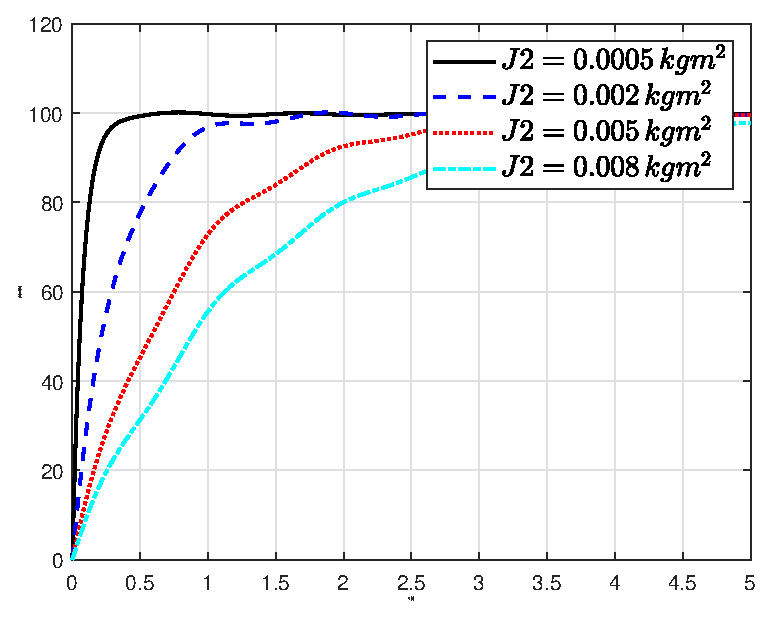
\includegraphics[width=\linewidth]{Bilder/5_sensi/fig/j2/phi_punkt.eps}
        \caption{Schwungrad Geschwindikeit}
        \label{fig:j2_phi_punkt}
    \end{subfigure}
    \begin{subfigure}[b]{0.49 \linewidth}
        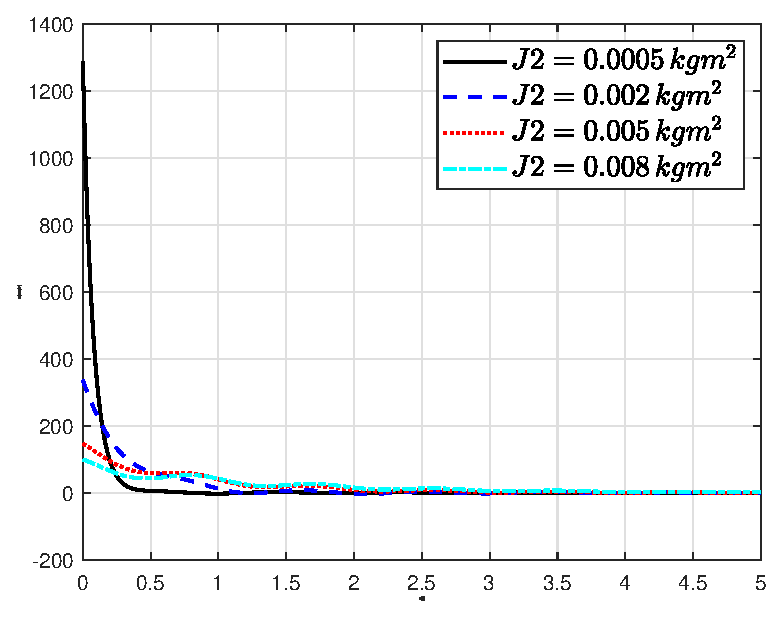
\includegraphics[width=\linewidth]{Bilder/5_sensi/fig/j2/phi_punkt_punkt.eps}
        \caption{Schwungrad Beschleunigung}
        \label{fig:j2_phi_punkt_punkt}
    \end{subfigure}
    \begin{subfigure}[b]{0.49 \linewidth}
        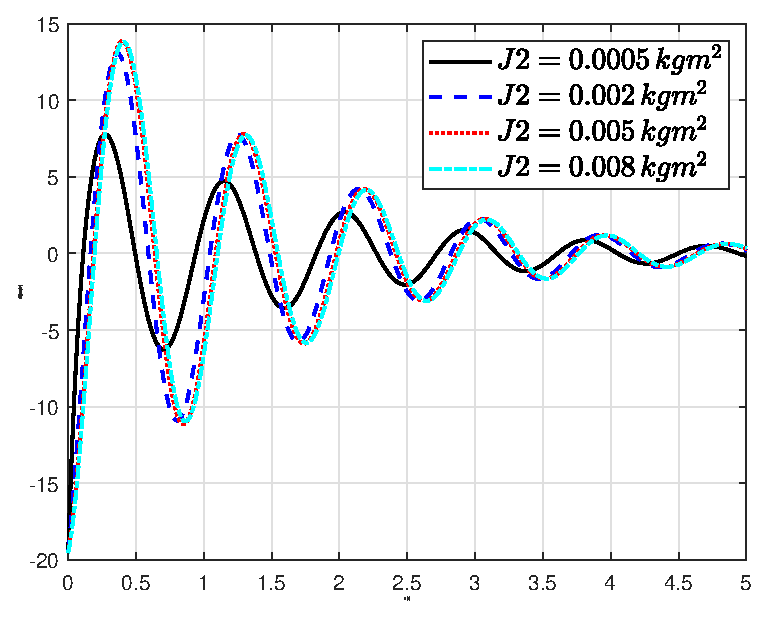
\includegraphics[width=\linewidth]{Bilder/5_sensi/fig/j2/theta_punkt_punkt.eps}
        \caption{Pendel Beschleunigung}
        \label{fig:j2_theta_punkt_punkt}
    \end{subfigure}
    \begin{subfigure}[b]{0.49\linewidth}
        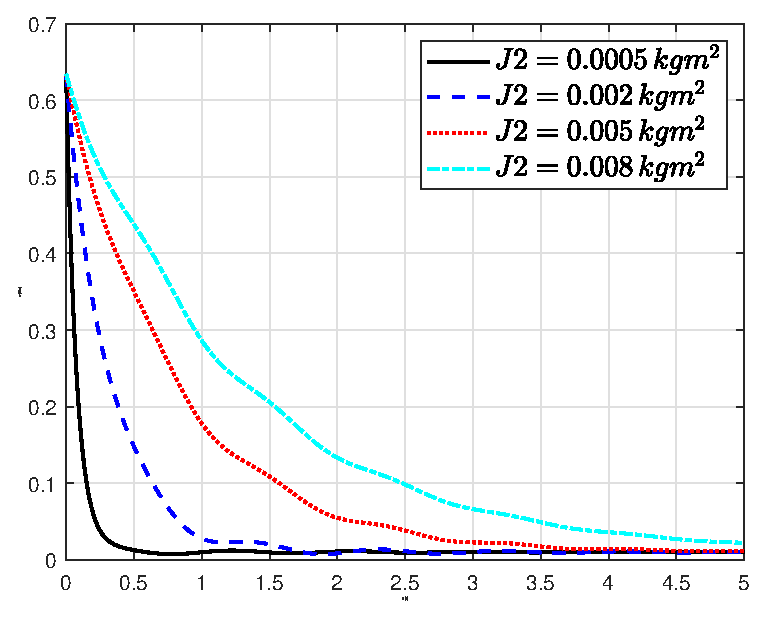
\includegraphics[width=\linewidth]{Bilder/5_sensi/fig/j2/tau.eps}
        \caption{Motor Moment}
        \label{fig:j2_tau}
    \end{subfigure}
    \begin{subfigure}[b]{0.49\linewidth}
        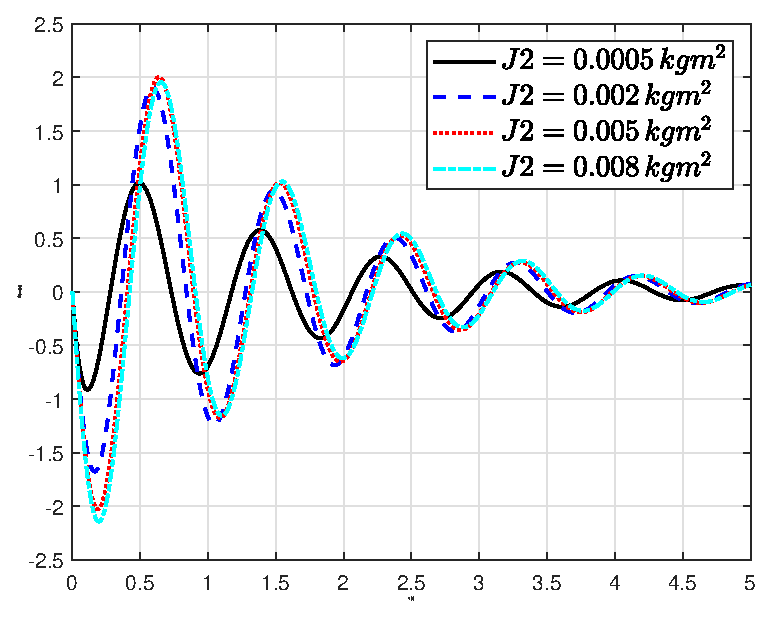
\includegraphics[width=\linewidth]{Bilder/5_sensi/fig/j2/theta_punkt.eps}
        \caption{Pendel Geschwindigkeit}
        \label{fig:j2_theta_punkt}      
    \end{subfigure}
    \begin{subfigure}[b]{0.49\linewidth}
        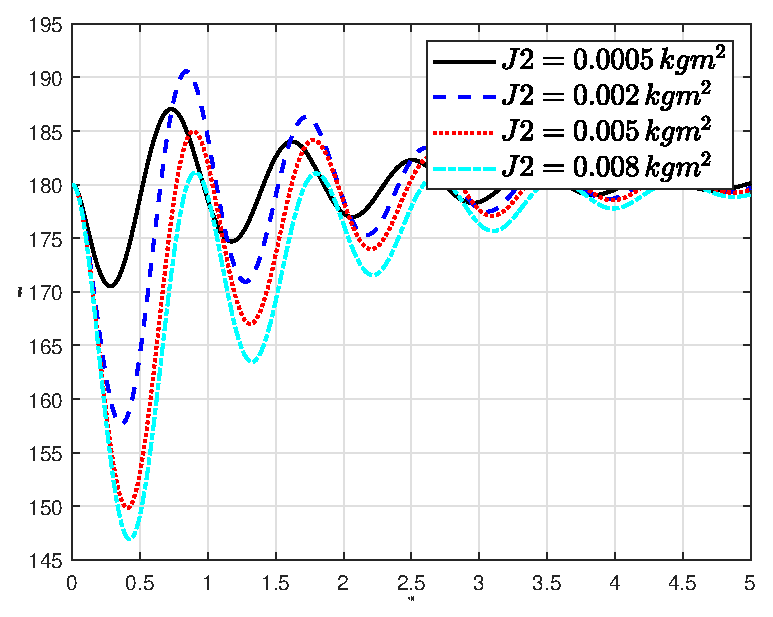
\includegraphics[width=\linewidth]{Bilder/5_sensi/fig/j2/theta.eps}
        \caption{Pendel Winkel}
        \label{fig:j2_theta}
    \end{subfigure}
        \caption{Modellantwort auf Varianz des Parameters: $J2$}
        \label{fig:j2}
\end{wrapfigure}
Die stationäre Endgeschwindigkeit des Schwungrades, wird durch den Parameter $J2$ stark beeinflusst (Abb. \ref{fig:j2_phi_punkt}). 
Bei erhöhter Trägheit des Schwungrades erhöht sich die Anstiegszeit, bis ein eingeschwungener Zustand erreicht wird.
Der Wert konvergiert allerdings bei allen Werten von $J2$ gegen die gleiche Endgeschwindigkeit.\\

Die Beschleunigung des Schwungrades wird ebenfalls stark beeinflusst (Abb. \ref{fig:j2_phi_punkt_punkt}).
Hierbei ist zu erkennen, dass ein erhöhtes Trägheitsmoment die maximale Beschleunigung bei $t\approx\SI{0}{\s}$ verringert. 
Ebenso wird der stationäre Zustand später erreicht und mit weiterer Erhöhung des Parameters ist ein Schwingen der Beschleunigung zu erkennen.\\
   
Das maximale Motormoment (Abb. \ref{fig:j2_tau}) ist bei allen Werten von $J2$ gleich, benötigt aber bei größeren Werten von $J2$ länger, um den stationären Zustand zu erreichen.\\
Dadurch, dass das Moment bei erhöhten Trägheitsmoment länger anliegt, wird auch eine größere Kraft auf das Pendel ausgeübt(Abb. \ref{fig:j2_theta_punkt_punkt}).\\
In Abb.\ref{fig:j2_theta} ist zu erkennen, dass ein größerer Winkelausschlag des Pendels erreicht wurde.\\
Dies ist ebenso der Fall bei der Pendelbeschleunigung (Abb. \ref{fig:j2_theta_punkt_punkt}) und der Pendelgeschwindigkeit (Abb. \ref{fig:j2_theta_punkt}).\\

 Das Trägheitsmoment des Schwungrades $J2$ hat also einen positiven Einfluss auf die Winkelantwort des Modells.\\  
 
 \subsection*{Einfluss der Masse des Schwungrads (M2)}
 Der Einfluss der Masse des Schwungrades ($m2$), auf die Modellparameter wird in den Simulationen (Abb. \ref{fig:m2}) untersucht. 
 Der Parameter $J2$ wird dabei von $\SI{0.01}{\kg}$ bis $\SI{1.5}{\kg}$ variiert.
 Die Motorspannung wird dabei auf \SI{10}{\volt} gesetzt und die anderen Parameter werden ebenfalls auf die Standardwerte in Tab. \ref{tab:Tabelle1.1} festgelegt.\\
 \begin{wrapfigure}{l}{0.5\textwidth}
    \captionsetup[subfigure]{justification=centering,font=footnotesize}
    \begin{subfigure}[b]{0.49\linewidth}
        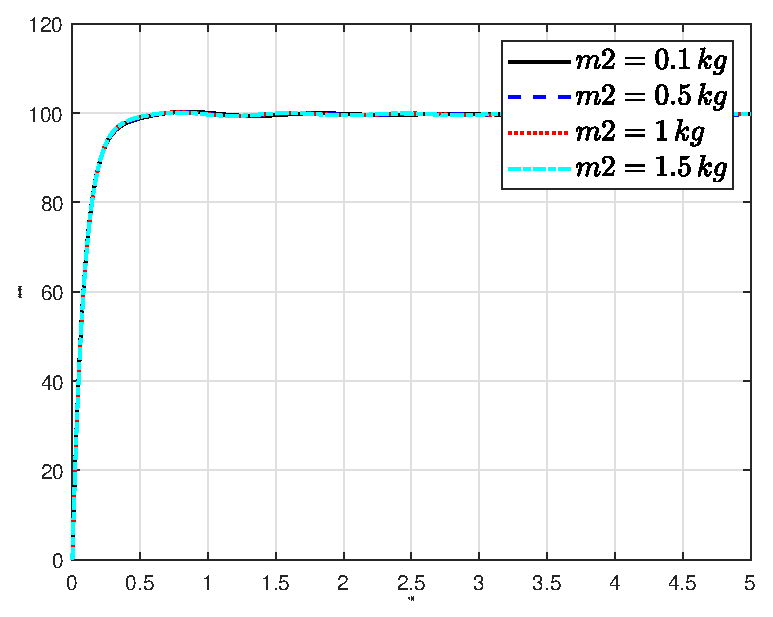
\includegraphics[width=\linewidth]{Bilder/5_sensi/fig/m2/phi_punkt.eps}
        \caption{Schwungrad Geschwindigkeit}
        \label{fig:m2_phi_punkt}
    \end{subfigure}
    \begin{subfigure}[b]{0.49 \linewidth}
        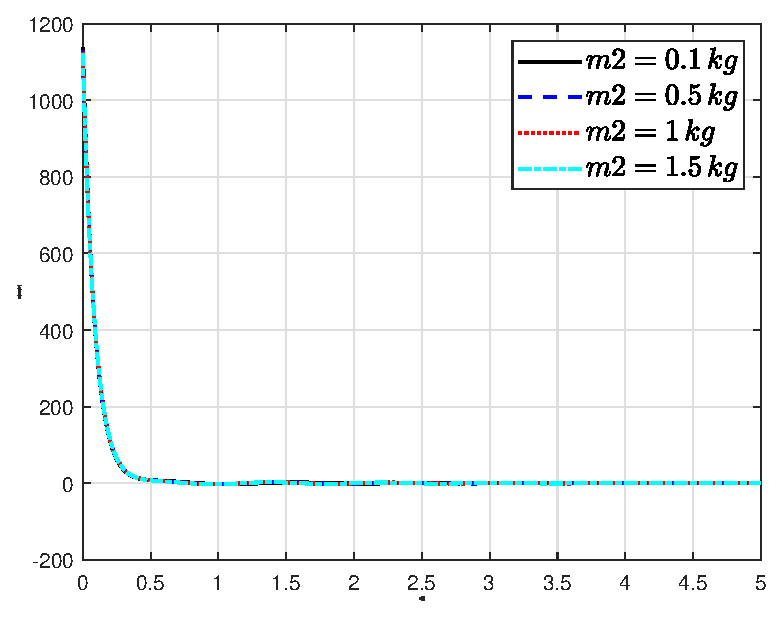
\includegraphics[width=\linewidth]{Bilder/5_sensi/fig/m2/phi_punkt_punkt.eps}
        \caption{Schwungrad Beschleunigung}
        \label{fig:m2_phi_punkt_punkt}
    \end{subfigure}
    \begin{subfigure}[b]{0.49 \linewidth}
        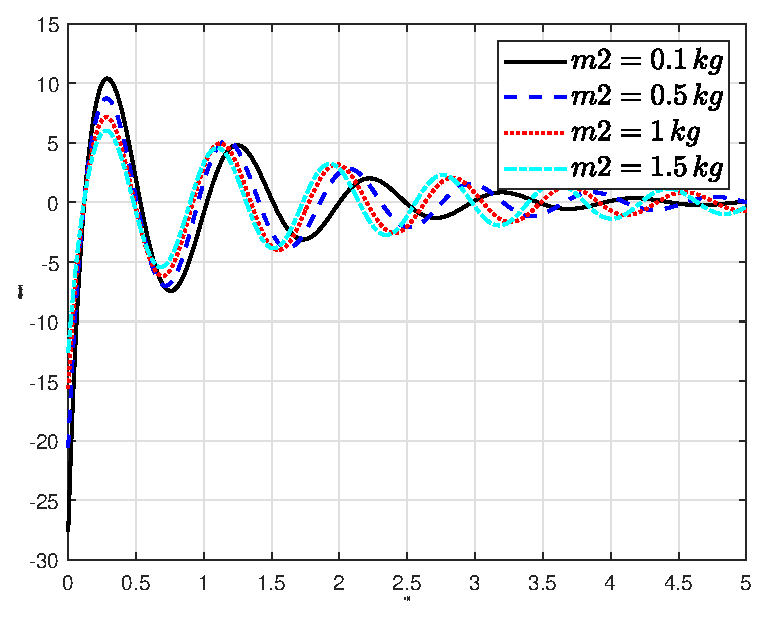
\includegraphics[width=\linewidth]{Bilder/5_sensi/fig/m2/theta_punkt_punkt.eps}
        \caption{Pendel Beschleunigung}
        \label{fig:m2_theta_punkt_punkt}
    \end{subfigure}
    \begin{subfigure}[b]{0.49\linewidth}
        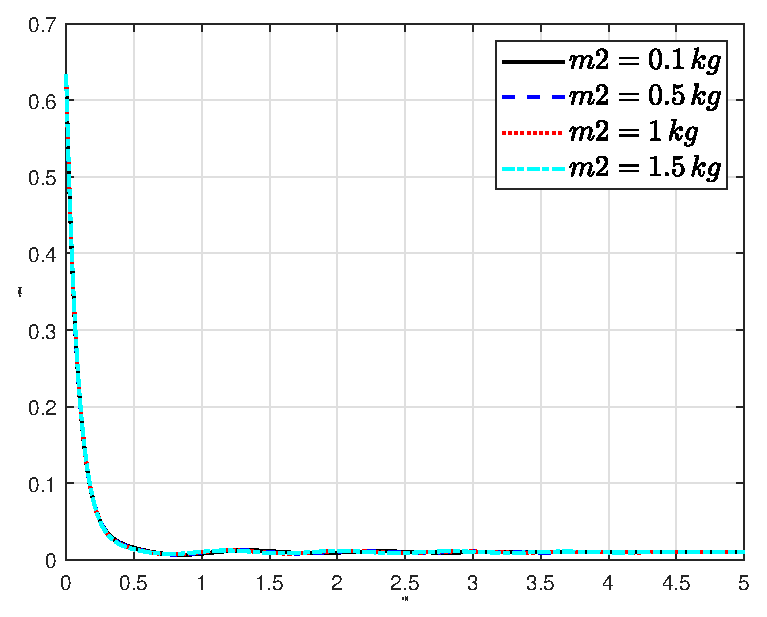
\includegraphics[width=\linewidth]{Bilder/5_sensi/fig/m2/tau.eps}
        \caption{Motor Moment}
        \label{fig:m2_tau}
    \end{subfigure}
    \begin{subfigure}[b]{0.49\linewidth}
        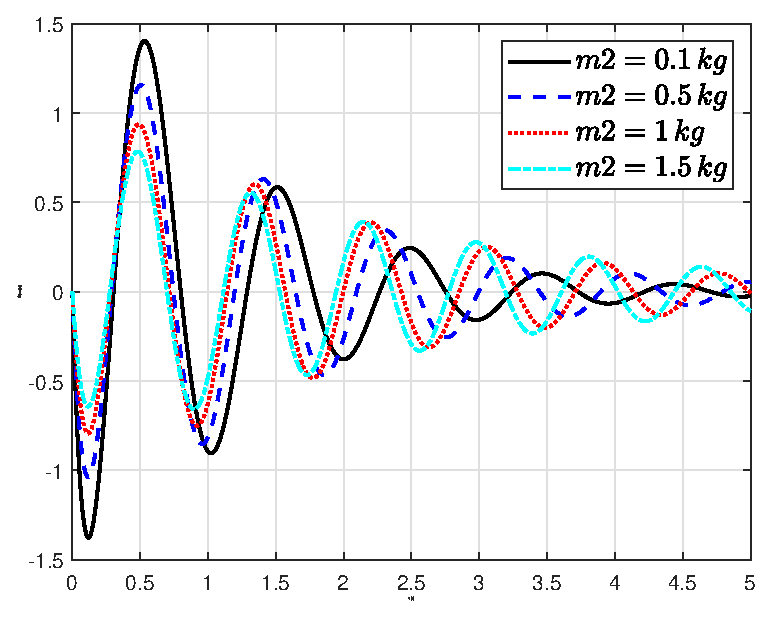
\includegraphics[width=\linewidth]{Bilder/5_sensi/fig/m2/theta_punkt.eps}
        \caption{Pendel Geschwindigkeit}
        \label{fig:m2_theta_punkt}      
    \end{subfigure}
    \begin{subfigure}[b]{0.49\linewidth}
        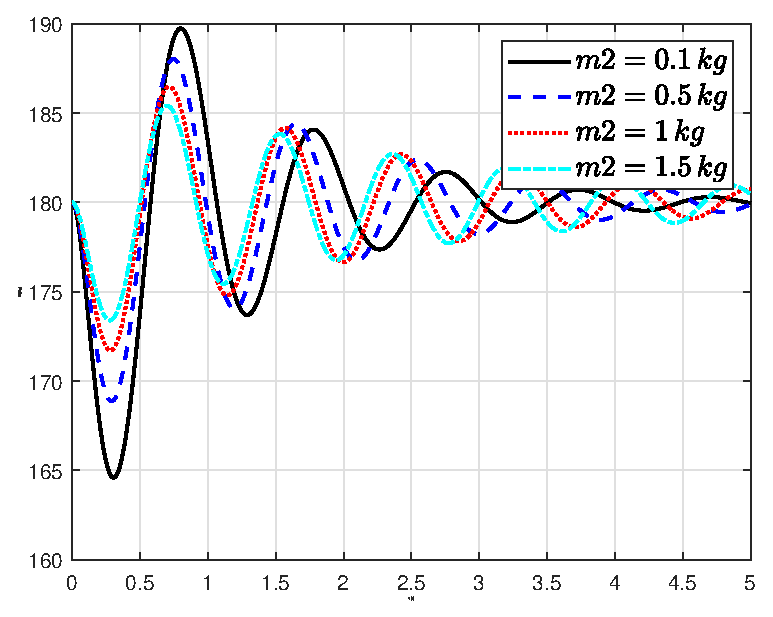
\includegraphics[width=\linewidth]{Bilder/5_sensi/fig/m2/theta.eps}
        \caption{Pendel Winkel}
        \label{fig:m2_theta}
    \end{subfigure}
        \caption{Modellantwort auf Varianz des Parameters: $M2$}
        \label{fig:m2}
\end{wrapfigure}
In den Simulationen ist zu erkennen, dass die Schwungradgeschwindigkeit (\ref{fig:m2_phi_punkt}), die Schwungradbeschleunigung (\ref{fig:m2_phi_punkt_punkt}) und das Motormoment (\ref{fig:m2_tau}) durch den Parameter $m2$ nicht beeinflusst werden.\\
Die Masse des Schwungrads hat also auf die gehaltenen Größen keinen Einfluss.\\

Der Winkel des Pendels (Abb. \ref{fig:m2_theta}) verringert sich mit Erhöhung der Masse $m2$. 
Dies ist auch bei der Pendelgeschwindigkeit (Abb. \ref{fig:m2_theta_punkt}) und der Pendelbeschleunigung (Abb. \ref{fig:m2_theta_punkt_punkt}) zu erkennen.\\
Dies liegt an der, durch die zusätzliche Masse, erhöhten Gewichtskraft, die auf das Pendel wirkt.\\
Ebenso wird die Dämpfung der Schwingung verändert und die Schwingungsdauer verlängert sich.\\

Die Erhöhung des Parameters $m2$ trägt also zu einer Verschlechterung der Modellantwort bei.

\subsection*{Einfluss der Reibung des Pendels (C1)}
Der Einfluss der Reibung des Pendels ($C1$), auf die Modellparameter wird in den Simulationen (Abb. \ref{fig:c1}) untersucht. 
Der Parameter $C1$ wird dabei von $\SI{0.01}{\newton\meter\second\per\radian}$ bis $\SI{1.5}{newton\meter\second\per\radian}$ variiert.
Die Motorspannung wird dabei auf \SI{10}{\volt} gesetzt und die anderen Parameter werden ebenfalls auf die Standardwerte in Tab. \ref{tab:Tabelle1.1} festgelegt.\\

 \begin{wrapfigure}{l}{0.5\textwidth}
    \captionsetup[subfigure]{justification=centering,font=footnotesize}
    \begin{subfigure}[b]{0.49\linewidth}
        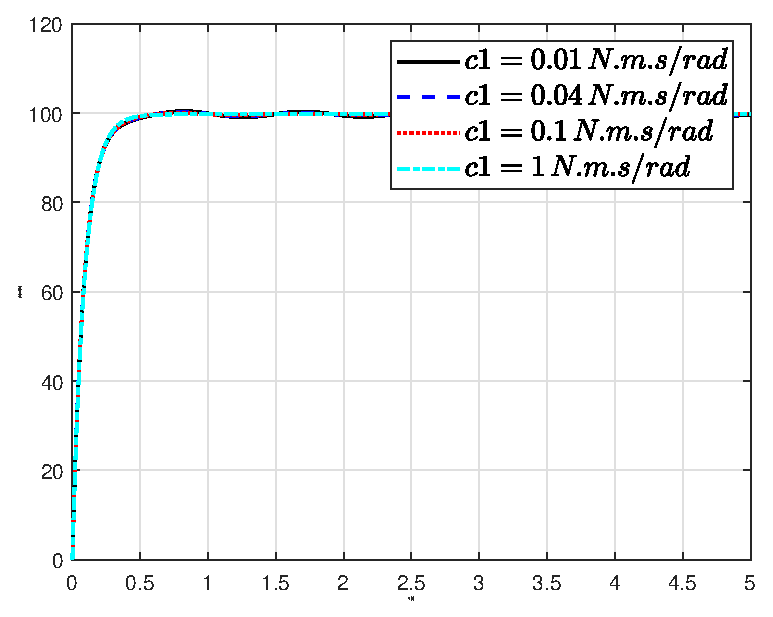
\includegraphics[width=\linewidth]{Bilder/5_sensi/fig/c1/phi_punkt.eps}
        \caption{Schwungrad Geschwindigkeit}
        \label{fig:c1_phi_punkt}
    \end{subfigure}
    \begin{subfigure}[b]{0.49 \linewidth}
        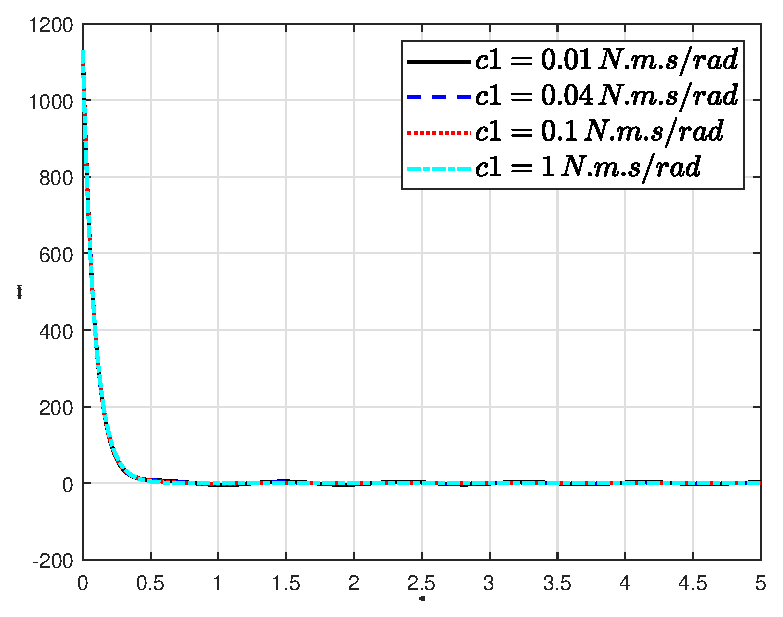
\includegraphics[width=\linewidth]{Bilder/5_sensi/fig/c1/phi_punkt_punkt.eps}
        \caption{Schwungrad Beschleunigung}
        \label{fig:c1_phi_punkt_punkt}
    \end{subfigure}
    \begin{subfigure}[b]{0.49 \linewidth}
        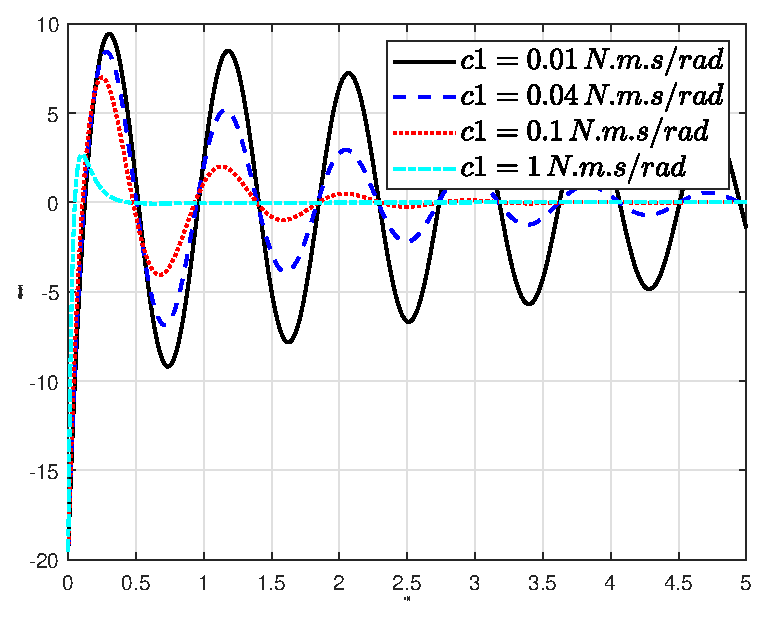
\includegraphics[width=\linewidth]{Bilder/5_sensi/fig/c1/theta_punkt_punkt.eps}
        \caption{Pendel Beschleunigung}
        \label{fig:c1_theta_punkt_punkt}
    \end{subfigure}
    \begin{subfigure}[b]{0.49\linewidth}
        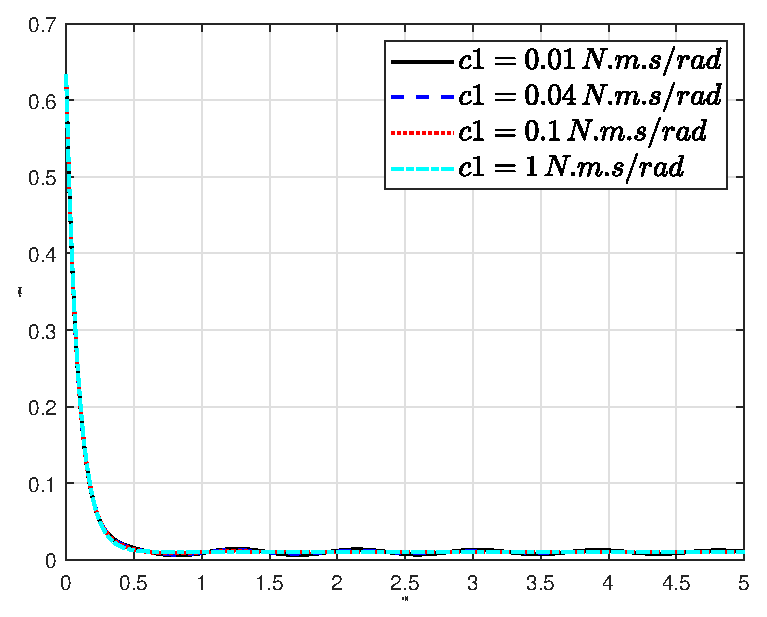
\includegraphics[width=\linewidth]{Bilder/5_sensi/fig/c1/tau.eps}
        \caption{Motor Moment}
        \label{fig:c1_tau}
    \end{subfigure}
    \begin{subfigure}[b]{0.49\linewidth}
        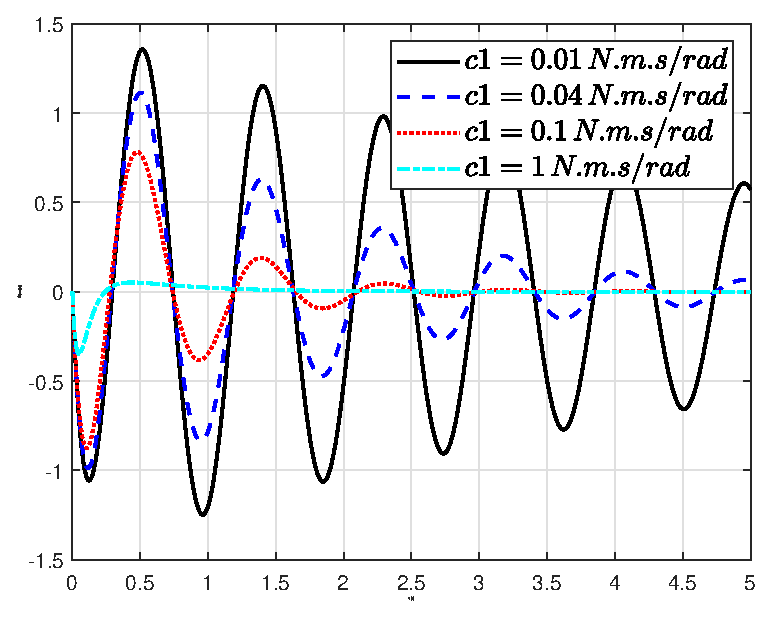
\includegraphics[width=\linewidth]{Bilder/5_sensi/fig/c1/theta_punkt.eps}
        \caption{Pendel Geschwindigkeit}
        \label{fig:c1_theta_punkt}      
    \end{subfigure}
    \begin{subfigure}[b]{0.49\linewidth}
        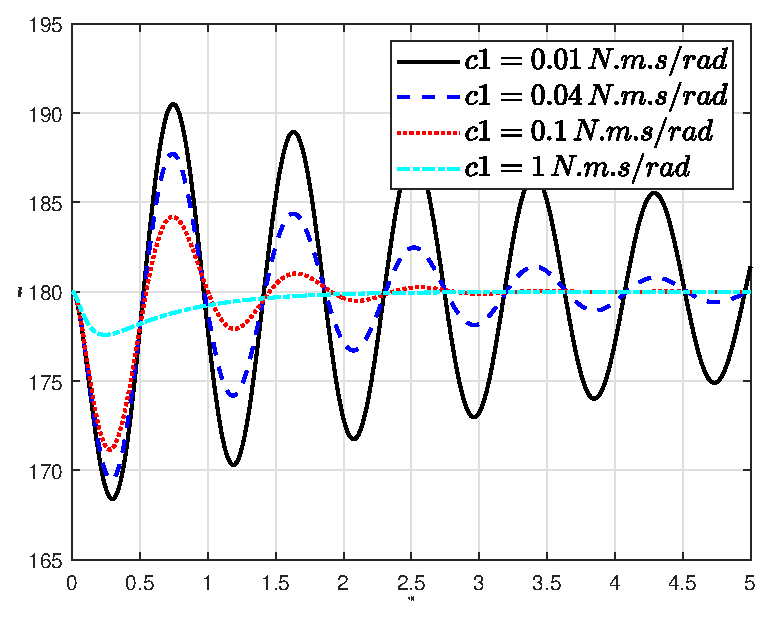
\includegraphics[width=\linewidth]{Bilder/5_sensi/fig/c1/theta.eps}
        \caption{Pendel Winkel}
        \label{fig:c1_theta}
    \end{subfigure}
        \caption{Modellantwort auf Varianz des Parameters: $C1$}
        \label{fig:c1}
\end{wrapfigure}

Die Schwungradgeschwindigkeit (Abb. \ref{fig:c1_phi_punkt}) und die Schwungradbeschleunigung (Abb. \ref{fig:c1_phi_punkt_punkt}) werden durch den Parameter $C1$ nicht beeinflusst.\\
Ebenso wird das Motormoment (\ref{fig:c1_tau}) durch die Reibung des Pendels nicht beeinflusst.\\

In der Pendelauslenkung (Abb. \ref{fig:c1_tau}) ist der Einfluss der Reibung deutlich zu erkennen. Je höher der Reibungskoeffizient, desto kleiner wird die Pendelauslenkung.\\
Ebenso wird, wie zu erwarten, die Pendelgeschwindigkeit (Abb. \ref{fig:c1_theta_punkt}) und die Pendelbeschleunigung (Abb. \ref{fig:c1_theta_punkt_punkt}) durch die Reibung des Pendels gedämpft.\\
Daraus lässt sich schließen, dass ein Teil des Momentes benötigt wird, um die Reibung zu überkommen. 

Die Erhöhung des Parameters $C1$ trägt also zu einer Verschlechterung der Modellantwort bei.
\subsection*{Einfluss der Reibung des Schwungrades (C2)}
Der Einfluss der Reibung des Schwungrades ($C2$), auf die Modellparameter wird in den Simulationen (Abb. \ref{fig:c2}) untersucht. 
Der Parameter $C2$ wird dabei von $\SI{0.0001}{\newton\meter\second\per\radian}$ bis $\SI{0.1}{\newton\meter\second\per\radian}$ variiert.
Die Motorspannung wird dabei auf \SI{10}{\volt} gesetzt und die anderen Parameter werden ebenfalls auf die Standardwerte in Tab. \ref{tab:Tabelle1.1} festgelegt.\\
 
\begin{wrapfigure}{l}{0.5\textwidth}
    \captionsetup[subfigure]{justification=centering,font=footnotesize}
    \begin{subfigure}[b]{0.49\linewidth}
        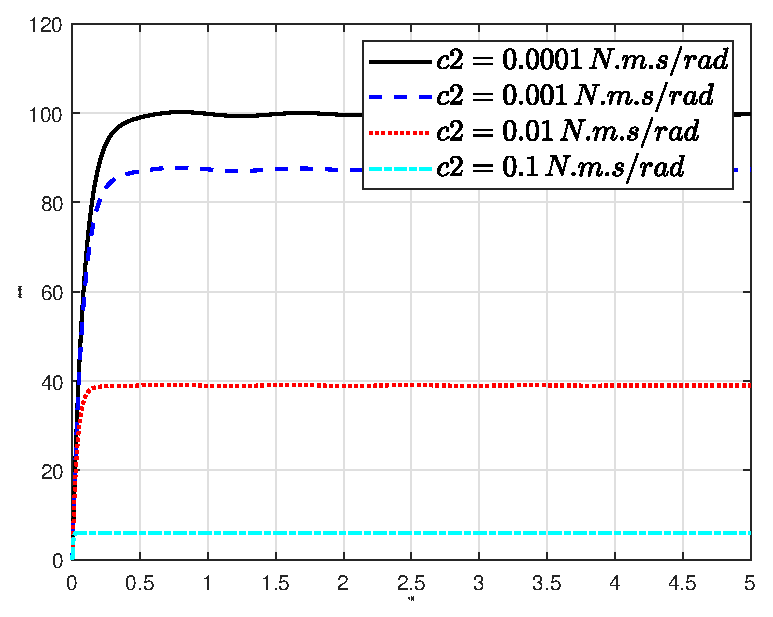
\includegraphics[width=\linewidth]{Bilder/5_sensi/fig/c2/phi_punkt.eps}
        \caption{Schwungrad Geschwindigkeit}
        \label{fig:c2_phi_punkt}
    \end{subfigure}
    \begin{subfigure}[b]{0.49 \linewidth}
        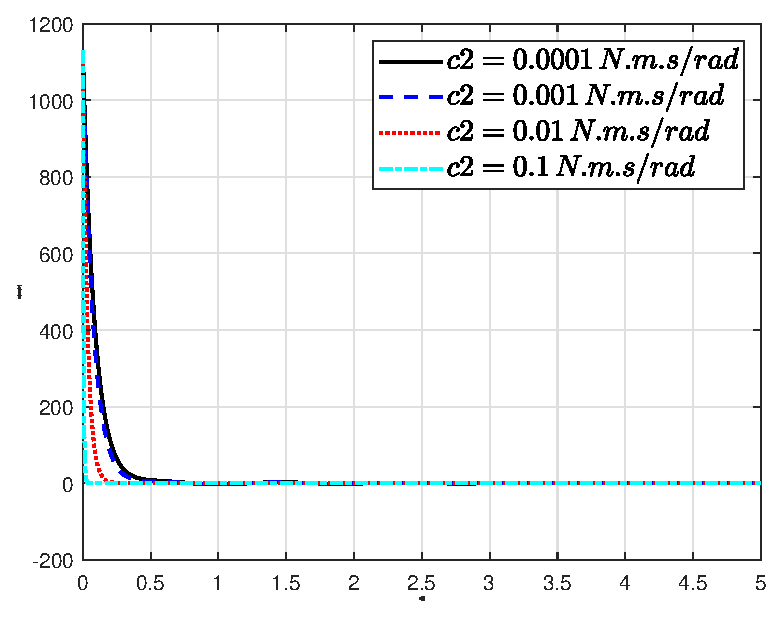
\includegraphics[width=\linewidth]{Bilder/5_sensi/fig/c2/phi_punkt_punkt.eps}
        \caption{Schwungrad Beschleunigung}
        \label{fig:c2_phi_punkt_punkt}
    \end{subfigure}
    \begin{subfigure}[b]{0.49 \linewidth}
        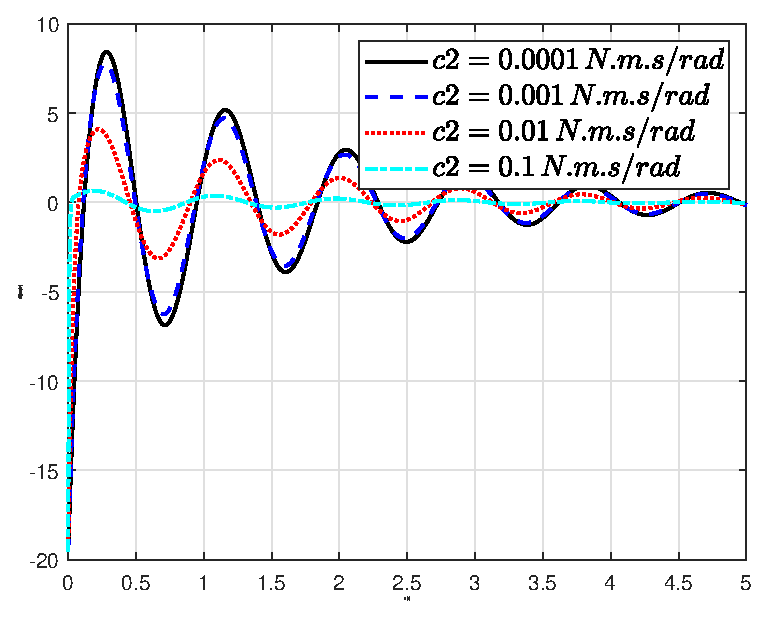
\includegraphics[width=\linewidth]{Bilder/5_sensi/fig/c2/theta_punkt_punkt.eps}
        \caption{Pendel Beschleunigung}
        \label{fig:c2_theta_punkt_punkt}
    \end{subfigure}
    \begin{subfigure}[b]{0.49\linewidth}
        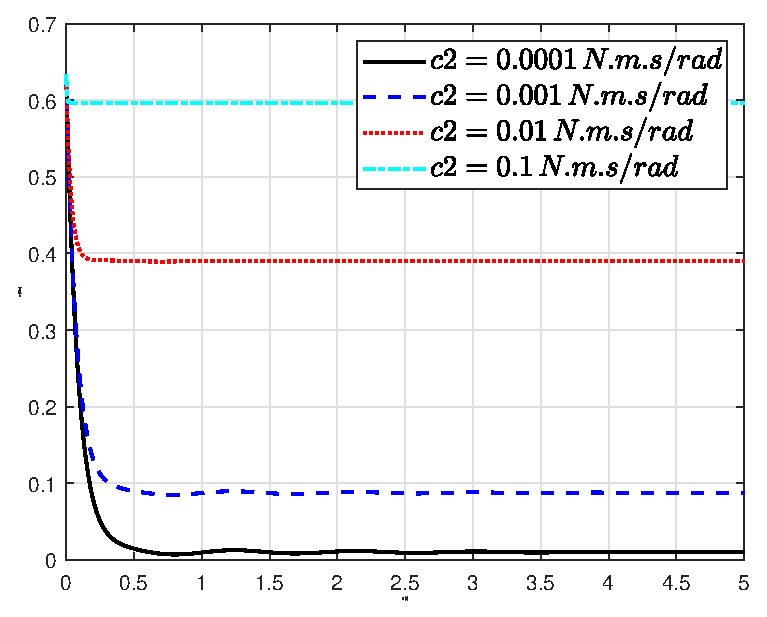
\includegraphics[width=\linewidth]{Bilder/5_sensi/fig/c2/tau.eps}
        \caption{Motor Moment}
        \label{fig:c2_tau}
    \end{subfigure}
    \begin{subfigure}[b]{0.49\linewidth}
        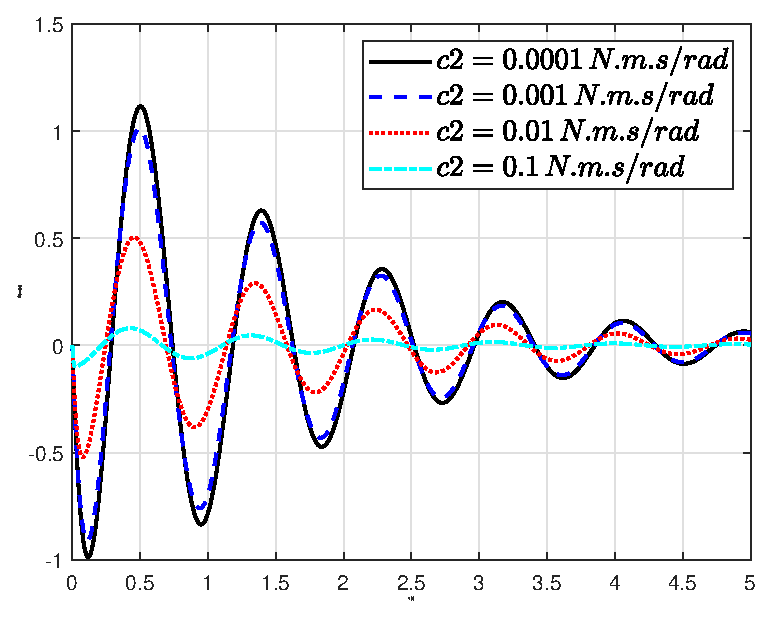
\includegraphics[width=\linewidth]{Bilder/5_sensi/fig/c2/theta_punkt.eps}
        \caption{Pendel Geschwindigkeit}
        \label{fig:c2_theta_punkt}      
    \end{subfigure}
    \begin{subfigure}[b]{0.49\linewidth}
        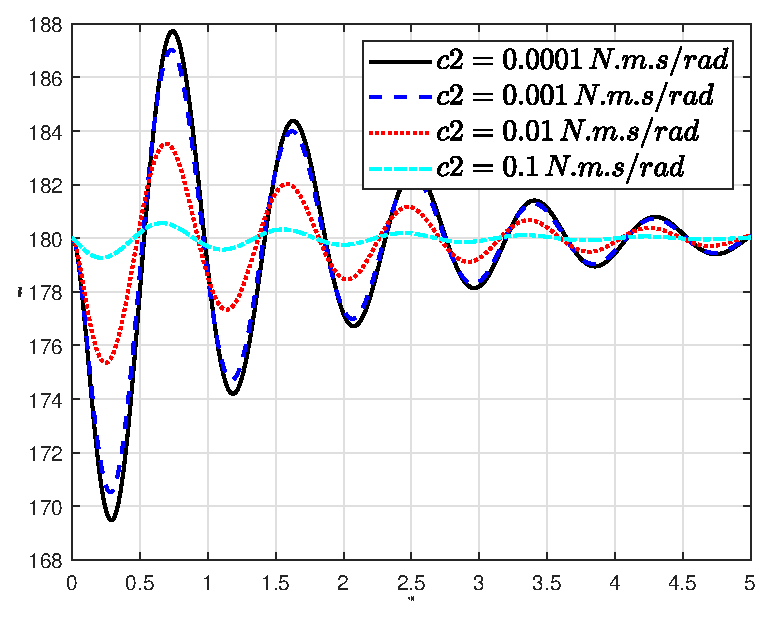
\includegraphics[width=\linewidth]{Bilder/5_sensi/fig/c2/theta.eps}
        \caption{Pendel Winkel}
        \label{fig:c2_theta}
    \end{subfigure}
        \caption{Modellantwort auf Varianz des Parameters: $C2$}
        \label{fig:c2}
\end{wrapfigure}

Die Schwungradgeschwindigkeit (Abb. \ref{fig:c2_phi_punkt}) wird durch die Reibung des Schwungrades stark beeinflusst. Je höher der Reibungskoeffizient, desto kleiner wird die maximale Schwungradgeschwindigkeit.\\
Die Reibung wirkt ebenfalls dämpfend auf Schwingung in der Geschwindigkeit und die Geschwindigkeit erreicht bei höher Reibung schneller ihren stabilen Endwert.\\

Die Schwungradbeschleunigung (Abb. \ref{fig:c2_phi_punkt_punkt}) wird ebenfalls durch die Reibung beeinflusst. Die maximale Beschleunigung um $t\approx\SI{0}{\s}$ ist unabhängig von $C2$, jedoch fällt sie schneller ab, je höher der Reibungskoeffizient ist.\\

Dadurch wird auch das Motormoment (Abb. \ref{fig:c2_tau}) beeinflusst. Je höher der Reibungskoeffizient, desto mehr Moment muss der Motor im stabilen Zustand aufbringen, um die Reibung zu überwinden.\\
Infolgedessen stellt sich ein konstantes Motormoment ein.

Das nun fehlende Motormoment macht sich auch in der Pendelgeschwindigkeit (Abb. \ref{fig:c2_theta_punkt}), der Pendelbeschleunigung (\ref{fig:c2_theta_punkt_punkt}) und dem Pendelwinkel (Abb. \ref{fig:c2_theta}) bemerkbar.\\
Je höher der Reibungskoeffizient $C2$ desto geringer die Amplituden.
Die Eigenfrequenz wird nicht beeinflusst.\\

Damit ist der Reibungskoeffizient $C2$ ein wichtiger Parameter, der alle wichtigen Modellgrößen beeinflusst.
\pagebreak
\subsection*{Überblick wichtiger Parameter und deren beinflusste Modellgrößen}
Im folgenden wird ein Überblick über die wichtigsten Parameter und deren beinflussten Modellgrößen gegeben.\\
Dabei handelt es sich um keine gewichtete Liste, sondern nur ein Überblcik aus den Parametern die die speziellen Modelgrößen Beinflussen.


\begin{minipage}[t]{.5\textwidth}
    \begin{itemize}
        \item Schwungradgeschwindigkeit $\dot\varphi$
        \begin{itemize}
            \item $V_m$
            \item $J2$
            \item $C2$
        \end{itemize}
        \item Schwungradbeschleunigung $\ddot\varphi$
        \begin{itemize}
            \item $V_m$
            \item $J2$
            \item $C2$
        \end{itemize}
        \item Pendelbeschleunigung $\ddot\Theta$
        \begin{itemize}
            \item $V_m$
            \item $l2$
            \item $J2$
            \item $m2$
            \item $C1$
            \item $C2$
        \end{itemize}
        \end{itemize}
\end{minipage}
\begin{minipage}[t]{.5\textwidth}
    \begin{itemize}
    \item Motormoment $\tau$
    \begin{itemize}
        \item $V_m$
        \item $J2$
        \item $C2$
    \end{itemize}
    \item Pendelgeschwindigkeit $\dot\Theta$
    \begin{itemize}
        \item $V_m$
        \item $l2$
        \item $J2$
        \item $m2$
        \item $C1$
        \item $C2$
    \end{itemize}
    \item Pendelwinkel $\Theta$
    \begin{itemize}
        \item $V_m$
        \item $l2$
        \item $J2$
        \item $m2$
        \item $C1$
        \item $C2$ 
    \end{itemize}
\end{itemize}
\end{minipage}

Besonders Wichtige Parameter sind:
\begin{itemize}
    \item Länge des Pendels zum Massenschwerpunkt $l2$
    \item Trägheitsmoment des Schwungrades $J2$
    \item Reibung des Schwungrades $C2$
    \item  Reibung des Pendels $C1$
\end{itemize}
All diese Parameter Beinflussen die wichtigsten Modelgrößen wie Pendelgeschwindigkeit, Pendelbeschleunigung und Pendelwinkel.\\

\section{Globale Sensitivitätsanalyse nach Monte Carlo Methode}
Bei der globale Sensitivitätsanalyse mit der Monte Carlo Methode werden die Parameter in einem bestimmten Bereich zufällig gewählt und die Modellgrößen berechnet.\\
Da es sich um eine Vielzahl von Paramter und Modellgrößen handelt, müssen viele Simulationen durchgeführt werden.\\
\begin{table}[H]
    \centering
    \begin{tabular}{|lll|}
        \hline
        \rowcolor{grey}
        \textbf{Symbol}     & \textbf{Parameter}                                & \textbf{Varianz der Parameter}                         \\ \hline
        $J_{\mathrm{1}}$    & Trägheitsmoment des Pendels (+ Motorstator)       & $\SI{0.01}{kg \cdot m^2}$ bis $\SI{0.1}{kg \cdot m^2}$                  \\
        $J_{\mathrm{2}}$    & Trägheitsmoment des Rads (+ Motorrotor)           & $\SI{0.0001}{kg \cdot m^2} $ bis $\SI{0.001}{kg \cdot m^2}$               \\
        $c_{\mathrm{1}}$    & Reibungsfaktor des Pendels                        & $\SI{0.04}{\frac{N \cdot m \cdot s}{rad}}$ bis $\SI{0.4}{\frac{N \cdot m \cdot s}{rad}}$    \\
        $c_{\mathrm{2}}$    & Reibungsfaktor des Rads                           & $\SI{0.0001}{\frac{N \cdot m \cdot s}{rad}}$ bis $\SI{0.001}{\frac{N \cdot m \cdot s}{rad}}$  \\
        $m_{\mathrm{1}}$    & Masse des Pendels und Stators                     & $\SI{0.8}{kg}$ bis $\SI{8}{kg}$                              \\
        $m_{\mathrm{2}}$    & Masse des Rads und Rotors                         & $\SI{0.5}{kg}$ bis $\SI{5}{kg}$                              \\
        $l_{\mathrm{1}}$    & Länge vom Ursprung bis Schwerpunkt des Pendels    & $\SI{0.1}{m}$ bis $\SI{1}{m}$                              \\
        $l_{\mathrm{2}}$    & Länge vom Ursprung bis Schwerpunkt des Rads       & $\SI{5}{V}$ bis $\SI{20}{V}$  \\
        $V_{\mathrm{m}}$    & Motorspannung       & $\SI{0.1}{m}$ bis $\SI{1}{m}$                                \\ \hline
    \end{tabular}
    \caption{Varianz der Modellparameter des Schwungrad-Pendels}
    \label{tab:varianz_parameter}
\end{table}

Über die in Tab. \ref{tab:varianz_parameter} aufgeführten Parameter wird eine Monte Carlo Simulation mit jeweils 1000 Zufallswerten pro Parameter durchgeführt.\\
Die Ergebnisse werden als Scatterplots dargestellt.\\

\begin{figure}
    \centering
    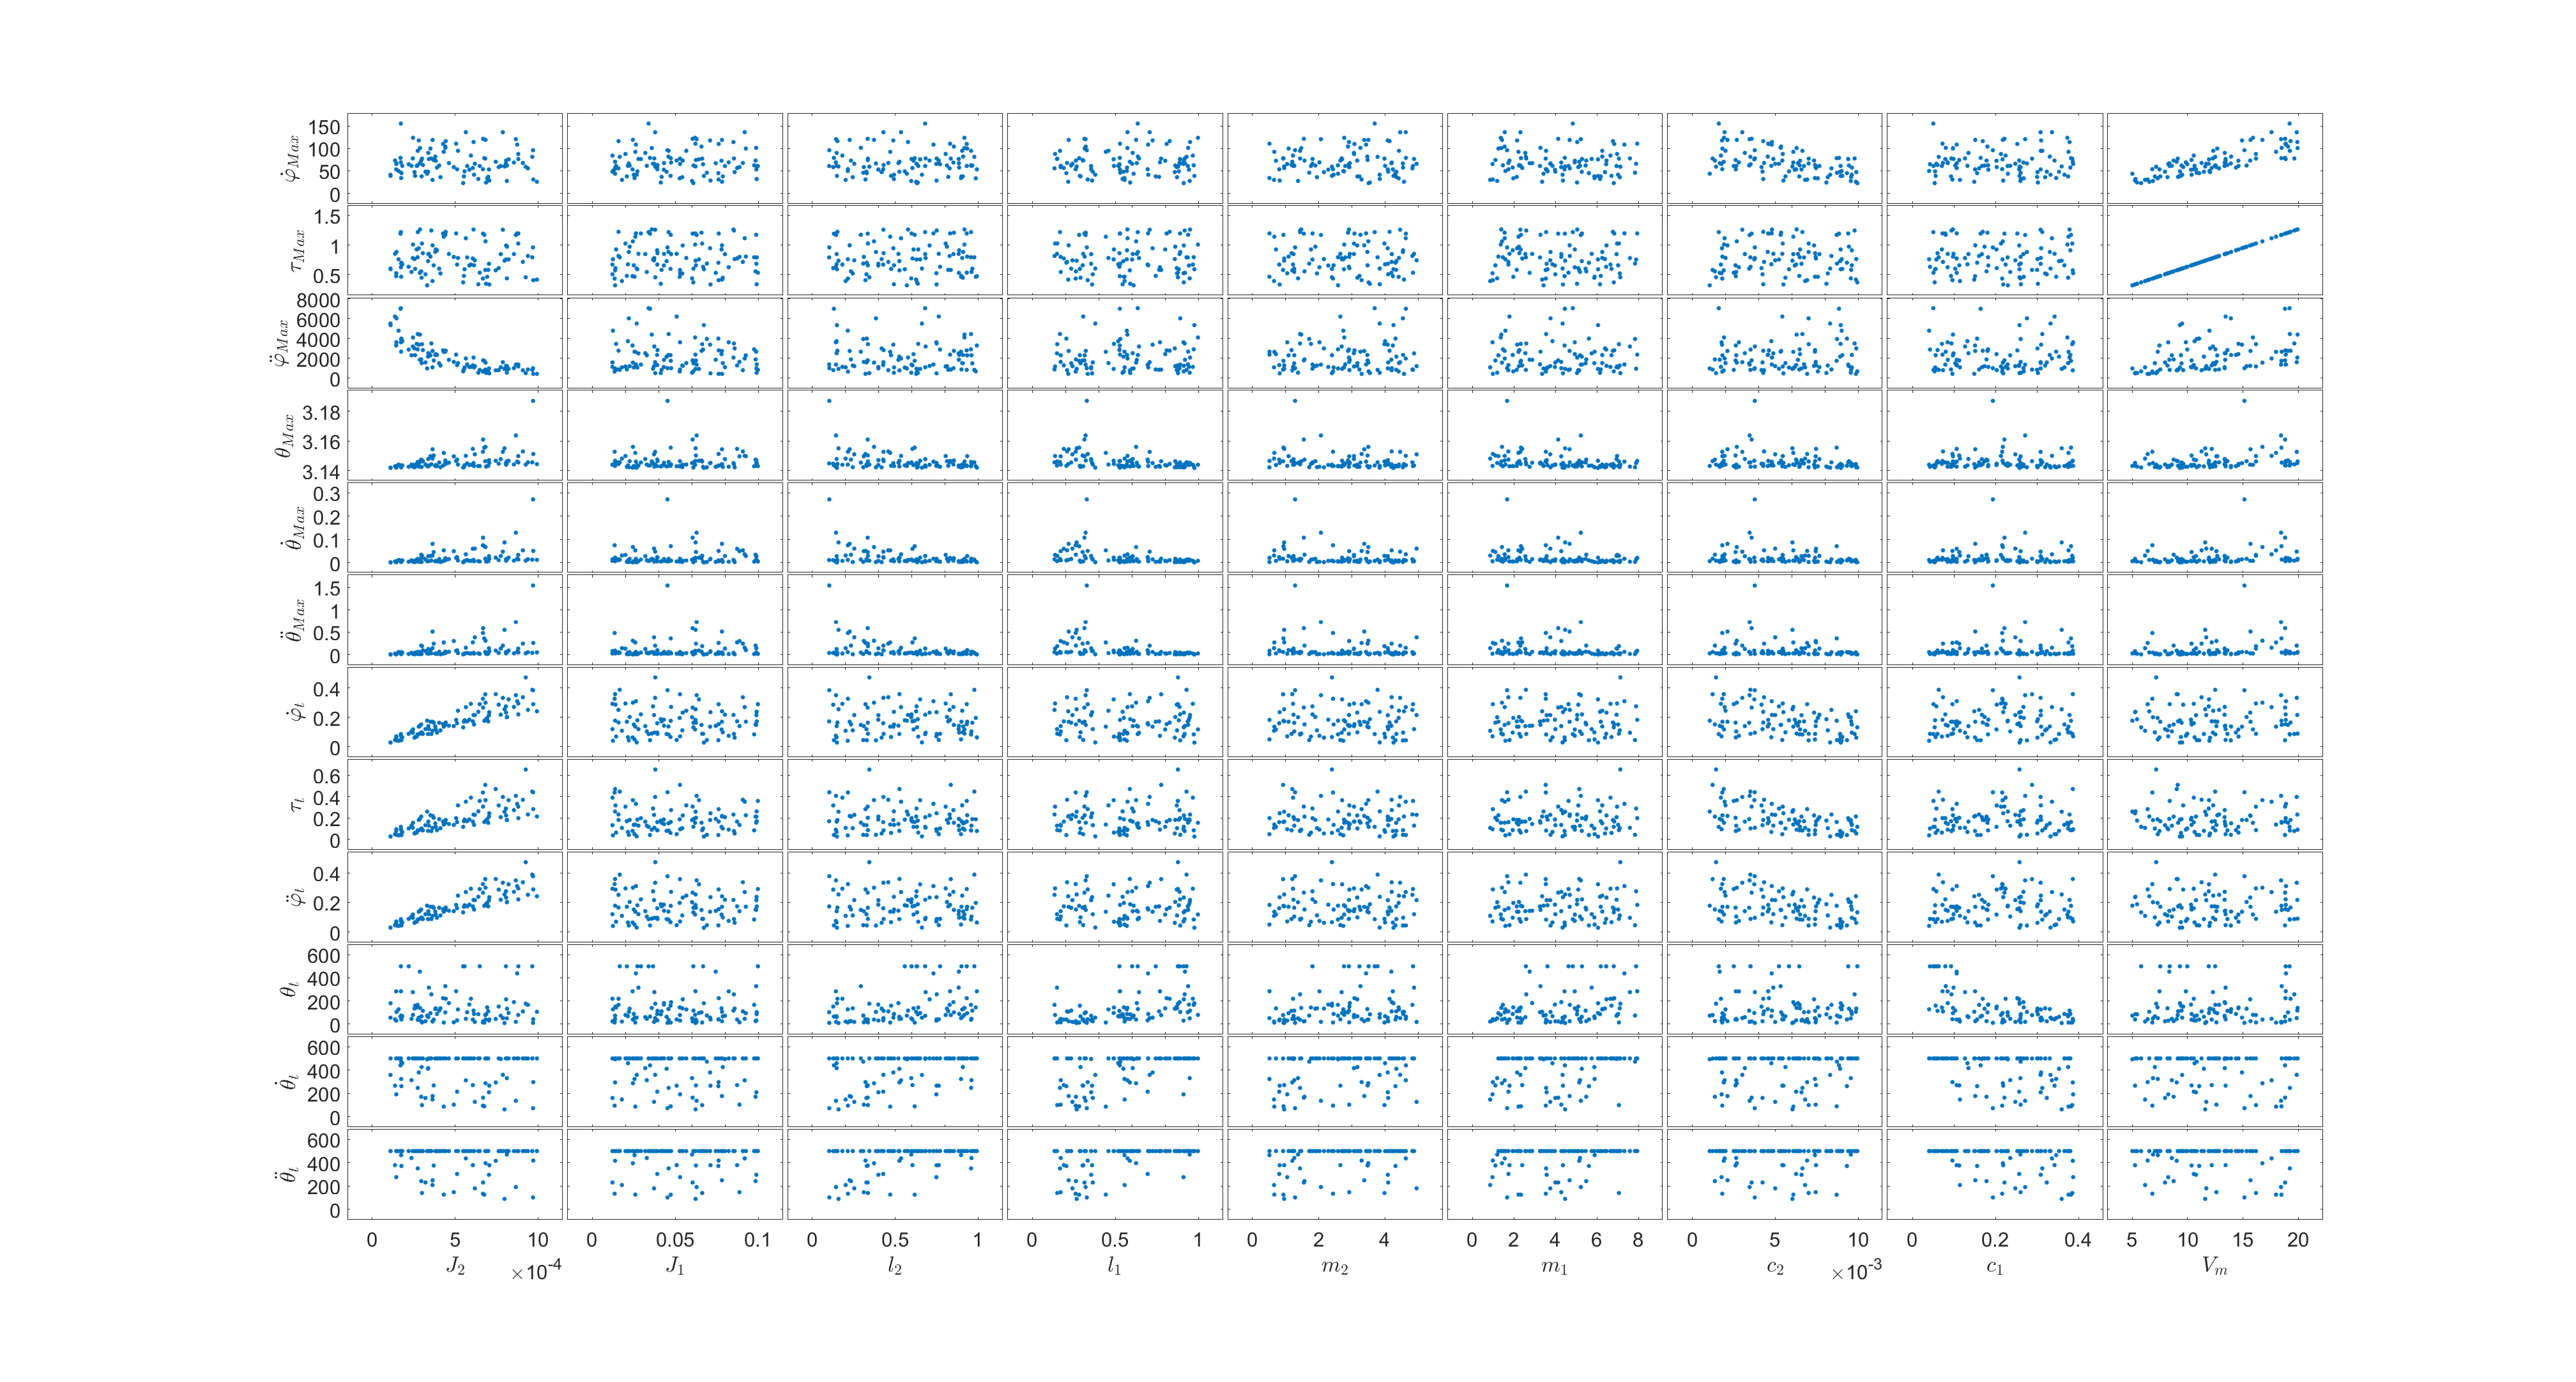
\includegraphics[width=\textwidth]{Bilder/5_sensi/cm/scatter.eps}
    \caption{Scatterplot über alle Parameter}
    \label{fig:scatter}
\end{figure}
Betrachtet man die Simulation über den gesammten Parameterraum (\ref{fig:scatter}), können einige eindeutige Korrelationen erkannt werden.
Bei Scatterplots ohne deutliche Korrelation lässt sich keine Beinflussung der Modellgrößen durch den gegebenen Parameter feststellen.

\subsection*{Schwungradgeschwindigkeit $\dot\varphi$}
$\bm{\dot\varphi}$ \textbf{max: }\\
Bei der maximalen Schwungradgeschwindigkeit gibt es zwei Parameter die die Modellgröße signifikant beeinflussen.\\
Dabei handelt es sich um die Motorspannung $V_{\mathrm{m}}$(Abb. \ref{fig:scatter_dotphi_max}) und die Reibung des Schwungrades $C_2$ (Abb. \ref{fig:scatter_dotphi_c2}).
Mit der definierten Varianz hat die Motorspannung einen größeren Einfluss, ist aber in Abhängigkeit von der Reibung des Schwungrades.\\

$\bm{\dot\varphi}$ \textbf{Settling Time: }\\
Bei der Settling Time gibt es zwei Parameter die  eine Korrelation erkennen lassen.
Das Trägheitsmoment des Schwungrades $J_2$ (Abb.\ref{fig:scatter_dotphi_t_j2}) ist positiv und die Reibung des Schwungrades $C_2$ (Abb.\ref{fig:scatter_dotphi_t_c2}) negativ mit der Einschwingzeit korreliert.
\begin{figure}
    \centering
    \begin{subfigure}[]{0.45\textwidth}
        \centering
        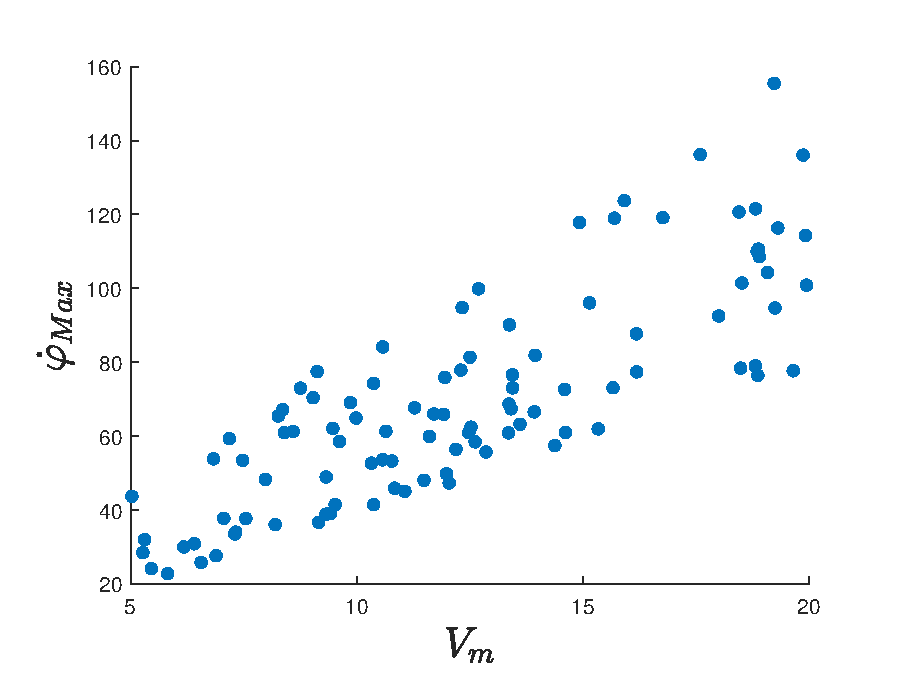
\includegraphics[width=\textwidth]{Bilder/5_sensi/cm/dot_phi_max.eps}
        \caption{Korrelation Motorspannung $V_m$}
        \label{fig:scatter_dotphi_max}
    \end{subfigure}
   \begin{subfigure}[]{0.45\textwidth}
        \centering
        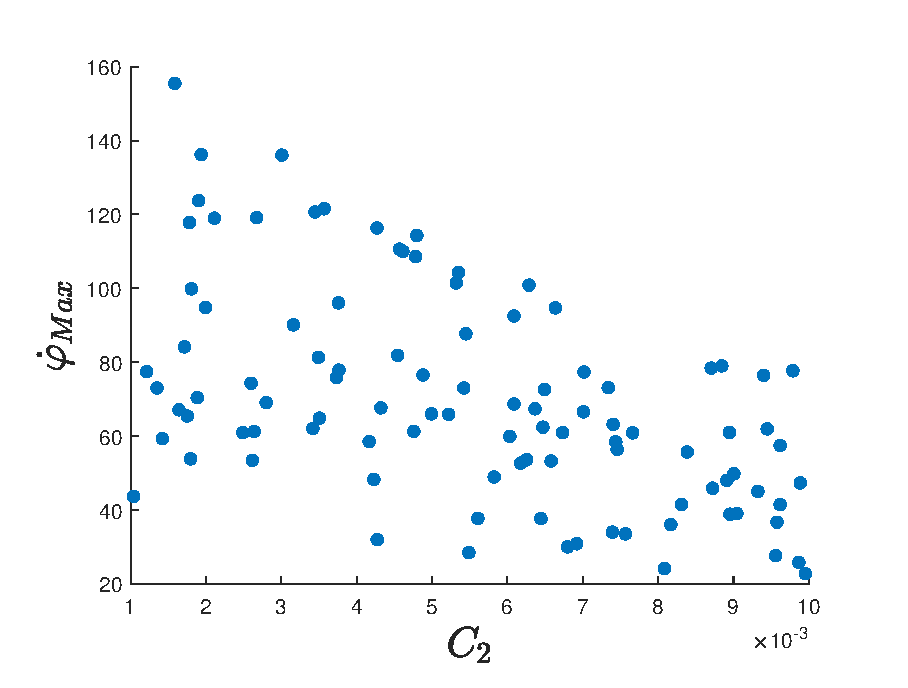
\includegraphics[width=\textwidth]{Bilder/5_sensi/cm/dot_phi_max_c2.eps}
        \caption{Korrelation Reibung $C_2$}
        \label{fig:scatter_dotphi_c2}
    \end{subfigure}
    \caption{Scatterplots über die maximale Schwungradgeschwindigkeit}
\end{figure}

\begin{figure}
    \centering
    \begin{subfigure}[]{0.45\textwidth}
        \centering
        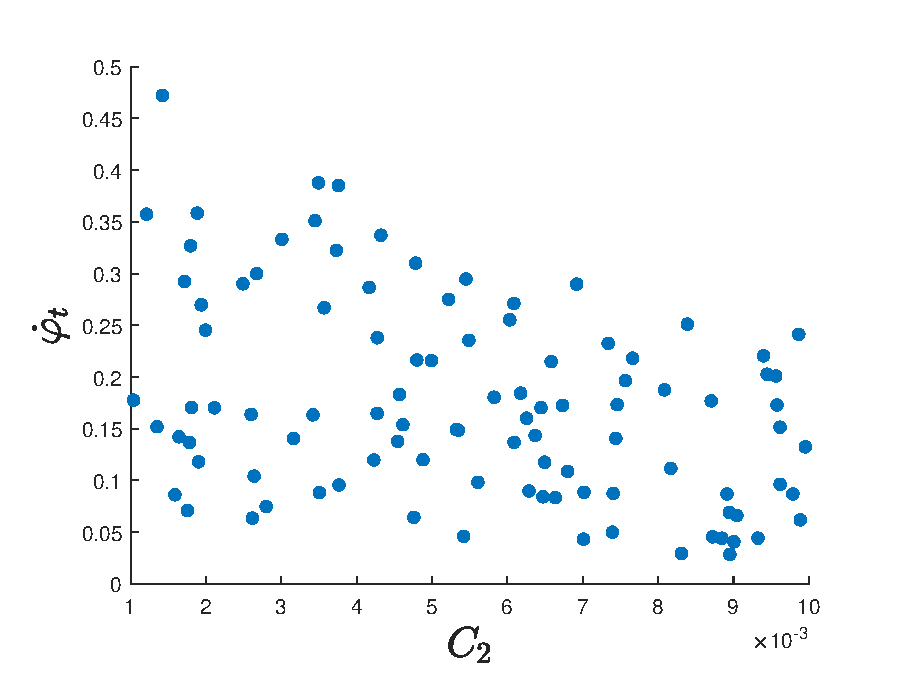
\includegraphics[width=\textwidth]{Bilder/5_sensi/cm/dot_phi_t_c2.eps}
        \caption{Korrelation Reibung $C_2$}
        \label{fig:scatter_dotphi_t_c2}
    \end{subfigure}
   \begin{subfigure}[]{0.45\textwidth}
        \centering
        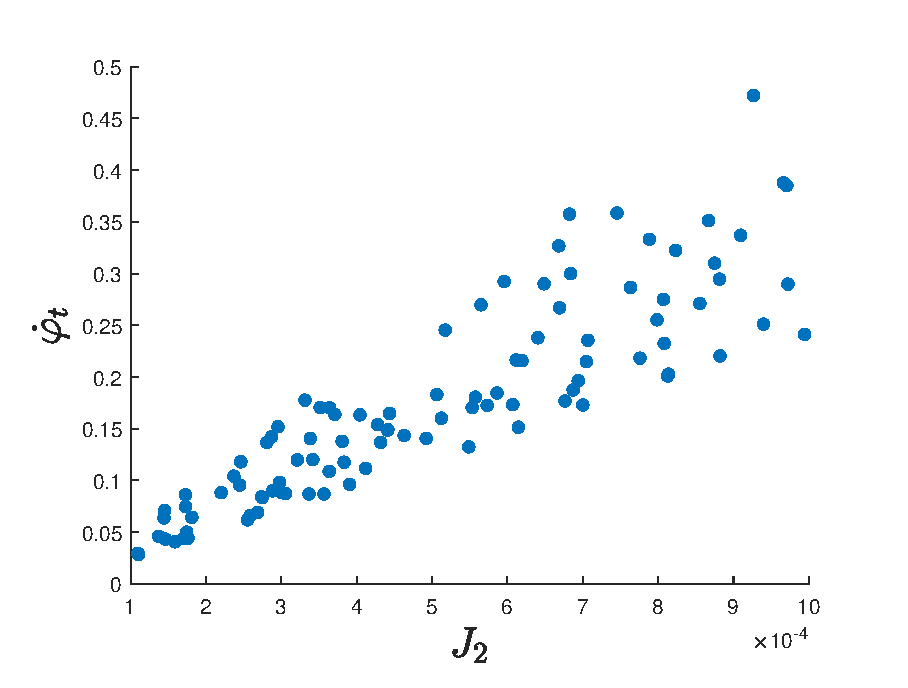
\includegraphics[width=\textwidth]{Bilder/5_sensi/cm/dot_phi_t_j2.eps}
        \caption{Korrelation Trägheitsmoment $J_2$}
        \label{fig:scatter_dotphi_t_j2}
    \end{subfigure}
    \caption{Scatterplots über die Einschwingzeit der Schwungradgeschwindigkeit}
\end{figure}
\subsection*{Schwungradbeschleunigung $\ddot\varphi$}
$\bm{\ddot\varphi}$ \textbf{max: }\\
Bei der maximalen Schwungradbeschleunigung gibt es eine deutlichhe Korrelation.
Das Trägheitsmoment des Schwungrades $J_2$ (Abb.\ref{scatter_dotdotphi_max_j2}) ist negativ mit der maximalen Schwungradbeschleunigung korreliert (Abb. \ref{}).\\

$\bm{\ddot\varphi}$ \textbf{Settling Time: }\\
Es gibt eine deutliche postitive korrelation zwischen dem Trägheitsmoment des Schwungrades $J_2$ und der Einschwingzeit der Schwungradbeschleunigung (Abb. \ref{fig:scatter_dodottphi_t_j2}).\\
Eine leicht negative Korrelation gibt es zwischen der Reibung des Schwungrades $C_2$ und der Einschwingzeit der Schwungradbeschleunigung (Abb. \ref{fig:scatter_dotdotphi_t_c2}).\\
\begin{figure}
    \centering
        \centering
        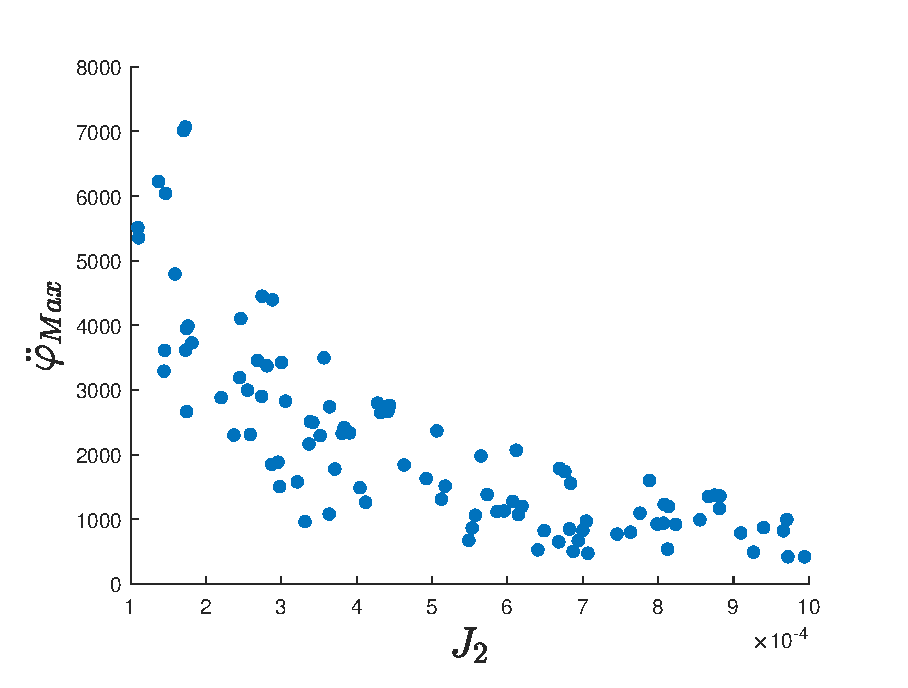
\includegraphics[width=0.5\textwidth]{Bilder/5_sensi/cm/dotdot_phi_max_J2.eps}
        \caption{Korrelation Trägheitsmoment $J_2$}
        \label{fig:scatter_dotdotphi_max_j2}
    \caption{Scatterplot über die maximale Schwungradbeschleunigung}
\end{figure}

\begin{figure}
    \centering
    \begin{subfigure}[]{0.45\textwidth}
        \centering
        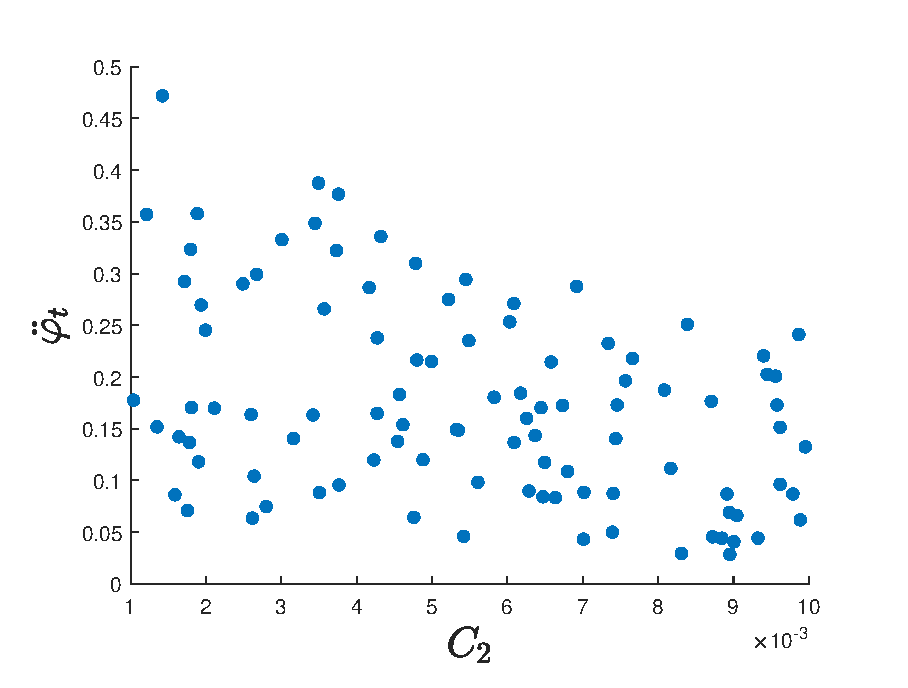
\includegraphics[width=\textwidth]{Bilder/5_sensi/cm/dotdot_phi_t_c2.eps}
        \caption{Korrelation Reibung $C_2$}
        \label{fig:scatter_dotdotphi_t_c2}
    \end{subfigure}
   \begin{subfigure}[]{0.45\textwidth}
        \centering
        \includegraphics[width=\textwidth]{Bilder/5_sensi/cm/dotdot_phi_t_j2.eps}
        \caption{Korrelation Trägheitsmoment $J_2$}
        \label{fig:scatter_dodottphi_t_j2}
    \end{subfigure}
    \caption{Scatterplots über die Einschwingzeit der Schwungradbeschleunigung}
\end{figure}
\subsection*{Pendelauslenkung $\Theta$}
$\bm{\Theta}$ \textbf{max: }\\
Das Trägheitsmoment des Schwungrades $J_2$ (Abb.\ref{fig:scatter_theta_max_j2}) sowie die Motorspannung $V_m$ (Abb. \ref{fig:scatter_theta_max_Vm}) sind positiv mit der maximalen Pendelauslenkung korreliert.\\
Die Länge $l_2$ ist neagitv mit der maximalen Pendelauslenkung korreliert (Abb. \ref{fig:scatter_theta_max_l2}).\\
$\bm{\Theta}$ \textbf{Settling Time: }\\
Bei der Pendeleinschwingzeit gibt es den negativ korrelierten Parameter \glqq Reibung des Pendels $C_1$\grqq{},
\begin{figure}
    \centering
    \begin{subfigure}[]{0.3\textwidth}
        \centering
        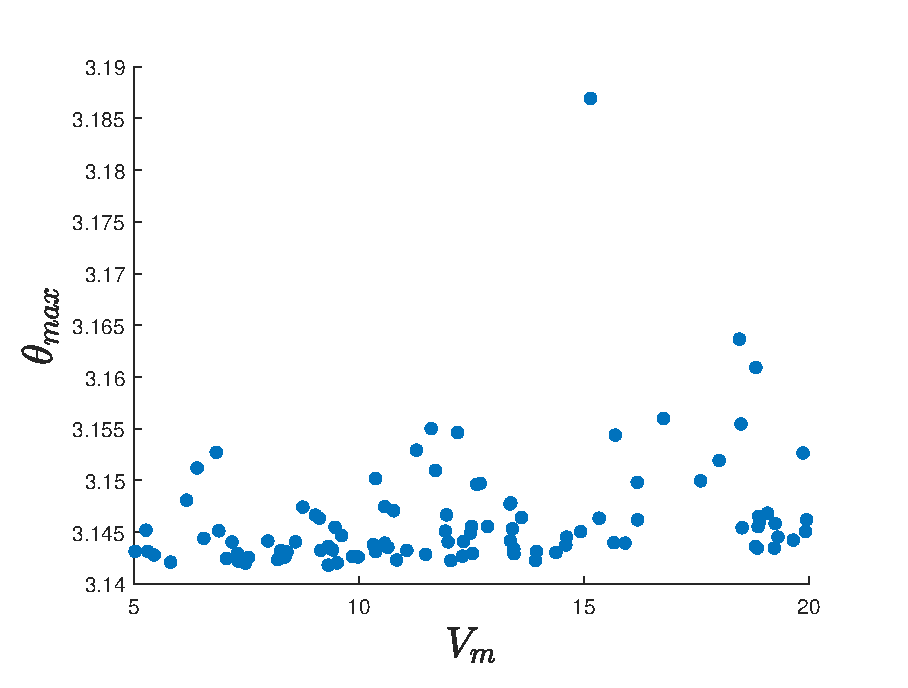
\includegraphics[width=\textwidth]{Bilder/5_sensi/cm/theta_max_Vm.eps}
        \caption{Korrelation Motorspannung $V_m$}
        \label{fig:scatter_theta_max_Vm}
    \end{subfigure}
   \begin{subfigure}[]{0.3\textwidth}
        \centering
        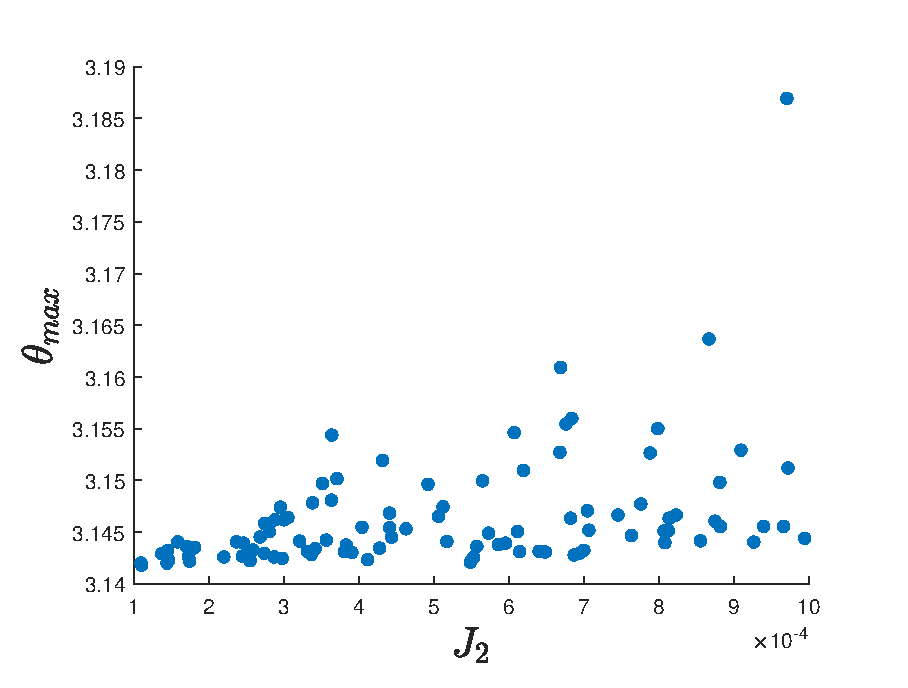
\includegraphics[width=\textwidth]{Bilder/5_sensi/cm/theta_max_j2.eps}
        \caption{Korrelation Trägheitsmoment $J_2$}
        \label{fig:scatter_theta_max_j2}
    \end{subfigure}
    \begin{subfigure}[]{0.3\textwidth}
        \centering
        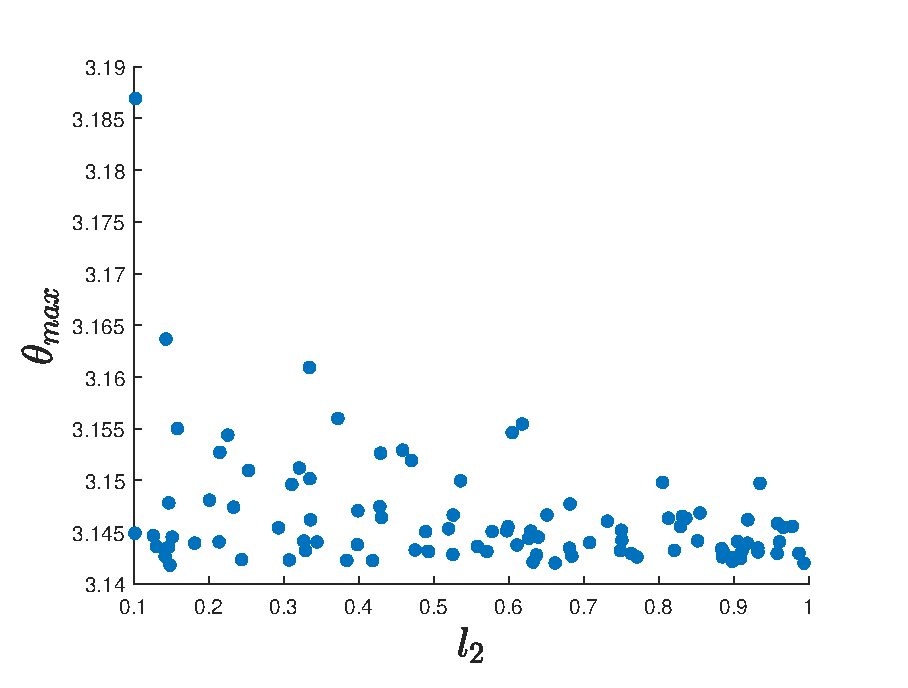
\includegraphics[width=\textwidth]{Bilder/5_sensi/cm/theta_max_l2.eps}
        \caption{Korrelation Länge $l_2$}
        \label{fig:scatter_theta_max_l2}
    \end{subfigure}
    \caption{Scatterplots über die maximale Pendelauslenkung}
\end{figure}

\begin{figure}
    \centering
        \centering
        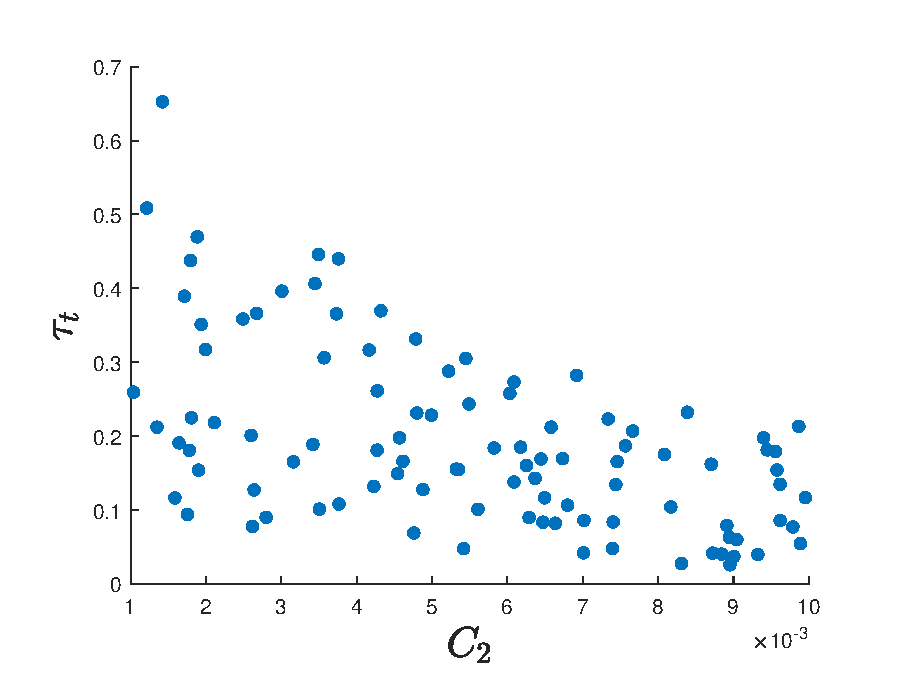
\includegraphics[width=0.5\textwidth]{Bilder/5_sensi/cm/theta_max_c1.eps}
        \caption{Korrelation Reibung $C_1$}
        \label{fig:scatter_theta_t_c1}
    \caption{Scatterplot über die Pendeleinschwingzeit}
\end{figure}

\subsection*{Pendelgeschwindigkeit $\dot\Theta$}
$\bm{\dot\Theta}$ \textbf{max: }\\
Es besteht eine positive Korrelation zwischen der maximalen Pendelgeschwindigkeit und dem Trägheitsmoment des Schwungrades $J_2$ (Abb. \ref{fig:scatter_dottheta_max_j2}).\\
$\bm{\dot\Theta}$ \textbf{Settling Time: }\\
Es lässt sich keine klare Korrelation erkennen.\\
\begin{figure}
        \centering
        \includegraphics[width=0.5\textwidth]{Bilder/5_sensi/cm/dot_theta_max_J2.eps}
        \caption{Korrelation Trägheitsmoment $J_2$}
        \label{fig:scatter_dottheta_max_j2}
    \caption{Scatterplot über die maximale Pendelgeschwindigkeit}
\end{figure}
\subsection*{Pendelbeschleunigung $\dddot\Theta$}
$\bm{\ddot\Theta}$ \textbf{max: }\\
Es besteht eine positive Korrelatin zwischen der maximalen Pendelbeschleunigung und dem Trägheitsmoment des Schwungrades $J_2$ (Abb. \ref{fig:scatter_dotdottheta_max_j2}).\\

$\bm{\ddot\Theta}$ \textbf{Settling Time: }\\
Es lässt sich keine klare Korrelation erkennen.\\
\begin{figure}
        \centering
        \includegraphics[width=0.5\textwidth]{Bilder/5_sensi/cm/dotdot_theta_max_J2.eps}
        \caption{Korrelation Trägheitsmoment $J_2$}
        \label{fig:scatter_dotdottheta_max_j2}
    \caption{Scatterplot über die maximale Pendelbeschleunigung}
\end{figure}
\subsection*{Motormoment $\tau$}
$\bm{\tau}$ \textbf{max: }\\Das maximale Motormoment ist positiv mit der Motorspannung $V_m$ (Abb. \ref{fig:scatter_tau_vmc}) korreliert.\\

$\bm{\tau}$ \textbf{Settling Time: }\\
Es besteht eine deutliche postitive Korrelation zwischen dem Trägheitsmoment des Schwungrades $J_2$ (Abb. \ref{fig:dotdot_phi_t_j2}) sowie eine neagtive Korrelation zwischen dem Reibungsfaktor $C_2$ (Abb. \ref{fig:scatter_tau_t_c2}) und der Einschwingzeit des Motormoments (Abb. \ref{}).\\
\begin{figure}
    \centering
        \centering
        \includegraphics[width=0.5\textwidth]{Bilder/5_sensi/cm/tau_max_vm.eps}
        \caption{Korrelation Motorspannung $V_m$}
        \label{fig:scatter_tau_vm}
    \caption{Scatterplot über das maximale Motormoment}
\end{figure}
 

\begin{figure}
    \centering
    \begin{subfigure}[]{0.45\textwidth}
        \centering
        \includegraphics[width=\textwidth]{Bilder/5_sensi/cm/dotdot_phi_t_c2.eps}
        \caption{Korrelation Reibung $C_2$}
        \label{fig:scatter_tau_t_c2}
    \end{subfigure}
   \begin{subfigure}[]{0.45\textwidth}
        \centering
        \includegraphics[width=\textwidth]{Bilder/5_sensi/cm/dotdot_phi_t_j2.eps}
        \caption{Korrelation Trägheitsmoment $J_2$}
        \label{fig:scatter_tau_t_j2}
    \end{subfigure}
    \caption{Scatterplots über die Einschwingzeit des Motormoments}
\end{figure}
